\documentclass[lettersize,journal]{IEEEtran}
\usepackage[utf8]{inputenc}
\usepackage{outlines}
\usepackage{graphicx}
\usepackage[inline]{enumitem}
\usepackage{wrapfig}
\usepackage{makecell}
\usepackage{pifont}% http://ctan.org/pkg/pifont
\usepackage{amsthm}
\usepackage{amsmath}
\usepackage{mathtools}
%\usepackage{amssymb}
\usepackage{stmaryrd} % Additional math symbols.
\usepackage{amsfonts}
\usepackage{flushend}
\usepackage{balance}
%\usepackage[hyphens]{url}
\usepackage{hyperref}
\usepackage{multicol}
\usepackage{multirow}
\usepackage{setspace} % For double, 1.5, single spacing etc.
\usepackage{xspace}
\usepackage{listings}
\usepackage{ifthen}
\usepackage{verbatim}
\usepackage{float} % Defines newfloat used below
\usepackage{subcaption}
\usepackage{microtype}
\usepackage{mathptmx} % Fails the display of parentheses in math environment
\usepackage{textcomp}
%\usepackage[sort&compress]{natbib}
\usepackage{booktabs}
\usepackage{longtable}
\usepackage{blindtext}
\usepackage{fancyhdr}
%These two let you use multibyte utf-8 characters, e.g. 03bb - λ 
\usepackage[mathletters]{ucs}
\usepackage[utf8]{inputenc}
\usepackage{wasysym}	% Defines \cent, \currency, \brokenvert
\usepackage{tikz}
\usepackage{esvect}
\usepackage{csquotes}
\usepackage{array}
\usepackage{xcolor, colortbl}
\usepackage{tablefootnote}
\usepackage{supertabular}
% hyperref redefines a number of macros, so it should be last.  Empirically,
% doing so eliminates compiler warnings.
%\usepackage[bookmarks, colorlinks, citecolor=green, urlcolor=blue, 
%                    filecolor=blue, linkcolor=blue]{hyperref}

% According to the hyperref readme, algorithm must follow hyperref
\usepackage{algorithm}
\usepackage{algorithmicx}
\usepackage{algpseudocode}

% for \newcolumntype macro
 \newcolumntype{L}{>{$}l<{$}}
 	\newcolumntype{C}{>{$}c<{$}}

% required for combined latex/pdf xfig figures
\DeclareGraphicsRule{.pdftex}{pdf}{.pdftex}{}


%~~~~~~~~~~~~~~~~~~~~~~~~~~~~~~~~~~~~~~~~~~~~~~~~~~~~~~~~~~~~~~~~~~~~~~~~~~~~~~
% Macros																{{{1

% English
\newcommand{\cf}{\hbox{\emph{cf.}}\xspace}
\newcommand{\deletia}{\ldots [deletia] \ldots}
\newcommand{\etal}{\hbox{\emph{et al.}}\xspace}
\newcommand{\eg}{\hbox{\emph{e.g.}}\xspace}
\newcommand{\ie}{\hbox{\emph{i.e.}}\xspace}
\newcommand{\scil}{\hbox{\emph{sc.}}\xspace} %scilicet: it is permitted to know
\newcommand{\st}{\hbox{\emph{s.t.}}\xspace}
\newcommand{\wrt}{\hbox{\emph{w.r.t.}}\xspace}
\newcommand{\etc}{\hbox{\emph{etc.}}\xspace}
\newcommand{\viz}{\hbox{\emph{viz.}}\xspace} %videlicet: it is permitted to see


% % Algorithms
% \newfloat{Protocol}{thp}{lop}
% \DeclareMathOperator{\cbar}{||} %denotes concurrency in protocol floats.
% \newfloat{Program}{thp}{lop}
% \newfloat{Procedure}{thp}{lop}
% \providecommand*{\algorithmautorefname}{Algorithm}

%~~~~~~~~~~~~~~~~~~~~~~~~~~~~~~~~~~~~~~~~~~~~~~~~~~~~~~~~~~~~~~~~~~~~~~~~~~~~~~
% Theorems, etc.														{{{2
%\newenvironment{proof-idea}{\noindent{\bf Proof Idea}\hspace*{1em}}{\bigskip}

%\theoremstyle{plain}
%\newtheorem{thm}{Theorem}[section]
%\newtheorem{lem}[thm]{Lemma}
%\newtheorem{prop}[thm]{Proposition}
%\newtheorem{cor}[thm]{Corollary}

\theoremstyle{remark}
\newtheorem*{rem}{Remark}

\theoremstyle{definition}
\newtheorem{defn}{Definition}[section]
\providecommand*{\defnautorefname}{Definition}
%\newtheorem{conj}{Conjecture}
%}}}~~~~~~~~~~~~~~~~~~~~~~~~~~~~~~~~~~~~~~~~~~~~~~~~~~~~~~~~~~~~~~~~~~~~~~~~~~~


%~~~~~~~~~~~~~~~~~~~~~~~~~~~~~~~~~~~~~~~~~~~~~~~~~~~~~~~~~~~~~~~~~~~~~~~~~~~~~~
% Aliases																{{{1
\newcommand{\infinity}{\infty}
%}}}~~~~~~~~~~~~~~~~~~~~~~~~~~~~~~~~~~~~~~~~~~~~~~~~~~~~~~~~~~~~~~~~~~~~~~~~~~~

%~~~~~~~~~~~~~~~~~~~~~~~~~~~~~~~~~~~~~~~~~~~~~~~~~~~~~~~~~~~~~~~~~~~~~~~~~~~~~~
% Missing unicode chars, other brokenness in ucs/inputenc {{{1
\DeclareUnicodeCharacter{183}{\cdot}						% ·
\DeclareUnicodeCharacter{931}{\ensuremath\Sigma}			% Σ
\DeclareUnicodeCharacter{9001}{\ensuremath\langle}			% 〈
\DeclareUnicodeCharacter{9002}{\ensuremath\rangle}			% 〉
\DeclareUnicodeCharacter{9608}{\ensuremath\blacksquare}		% █
\DeclareUnicodeCharacter{1013}{\in}							% ϵ
\DeclareUnicodeCharacter{8213}{---}							% ―

\renewcommand{\textcent}{\cent}
\renewcommand{\textcurrency}{\currency}
\renewcommand{\textyen}{\yen}
\renewcommand{\textbrokenbar}{\brokenvert}
%}}}~~~~~~~~~~~~~~~~~~~~~~~~~~~~~~~~~~~~~~~~~~~~~~~~~~~~~~~~~~~~~~~~~~~~~~~~~~~

\usepackage{framed}
\newcounter{RQCounter}
\newcommand{\RQ}[1]{%
	\stepcounter{RQCounter}
	\begin{framed}%
		\noindent\textbf{Research Question \arabic{RQCounter}: }%
		#1\end{framed}
}

\newcommand{\cmark}{\ding{51}}%
\newcommand{\xmark}{\ding{55}}%

\DeclareTextFontCommand{\findings}{\normalfont\itshape\bfseries}

\newlength{\emstr}
\setlength{\emstr}{0.75em plus 1ex minus 1ex}
\newcommand{\boldpara}[1]{%
	\smallskip%
	\par\noindent\textbf{\textit{#1}}\hspace{\emstr}
}%

\def\sectionautorefname{Section}
\def\subsectionautorefname{Section}
\def\subsubsectionautorefname{Section}

% vim:foldmethod=marker

%%%%%%%%%%%%%%%%%%%%%%%%%%%%%%%%% Comments %%%%%%%%%%%%%%%%%%%%%%%%%%%%%
\newboolean{showcomments}
\setboolean{showcomments}{true} % comment this line to deactivate comments
\ifthenelse{\boolean{showcomments}}{
  \newcommand{\nbc}[3]{
    {\colorbox{#3}{\bfseries\sffamily\scriptsize\textcolor{white}{#1}}}%
    {\textcolor{#3}{\sf\small
    %$\blacktriangleright$
    \textit{#2}
    %$\blacktriangleleft$
    }}}
  \newcommand{\todo}[1]{\nbc{TODO}{#1}{blue}\xspace}
  \newcommand{\mar}[1]{\nbc{MAR}{#1}{cyan}\xspace}
  \newcommand{\earl}[1]{\nbc{EARL}{#1}{teal}\xspace}
  \newcommand{\fe}[1]{\nbc{FEDERICA}{#1}{violet}\xspace}
  \newcommand{\carlos}[1]{\nbc{CARLOS}{#1}{olive}\xspace}
}{
  \newcommand{\nbc}[3]{}
  \newcommand{\todo}[1]{}
  \newcommand{\mar}[1]{}
  \newcommand{\earl}[1]{}
  \newcommand{\fe}[1]{}
  \newcommand{\carlos}[1]{}
}


\newcommand{\ApproachName}{{\sc Imhotep}}
\newcommand{\CaseStudy}{Kromaia}

\title{Automated Software Transplantation on Procedural Content Generation}
\author{Mar Zamorano, Carlos Cetina, Federica Sarro}

\begin{document}

\maketitle

\begin{abstract}
Procedural Content Generation (PCG) aims for the (semi) automatic generation of new content within video games. However, usually the developers have limited control over the generation process.
We propose the first transplantation algorithm in the field of PCG that allows game developers to choose an organ from a donor and a host that will receive the organ. Through our approach, we aim to search for an appropriate solution to integrate the organ into the host. We also study two distinct objective functions: the one accepted in the literature of  software transplantation (test-based variant), and a novel objective function (simulation-based variant).
In our evaluation, we have transplanted a total of 129 distinct organs from the scenarios of \CaseStudy{} (a commercial video game) into 5 video game bosses as hosts.
Our simulation-based variant produces results that are 1.5 times superior to those of the test-based variant and 2.5 times superior to the PCG baseline. The statistical analysis confirms the significance of these differences and highlights the substantial magnitude of improvement.
Furthermore, a focus group with game developers indicated their satisfaction with the generated content.
Our analysis of the results also reveals organ interactions that have not been  identified previously in the literature.
\end{abstract}

\begin{IEEEkeywords}
Automated Software Transplantation, Auto-transplantation, Procedural Content Generation, Search-Based Software Engineering, Model-Driven Engineering
\end{IEEEkeywords}

\section{Introduction}
\label{sec:intro}

%\IEEEPARstart{T}{he} 

The video games industry grows significantly every year~\cite{rykala2020growth}. In 2019, it became the largest entertainment industry in terms of revenue after surpassing the combined revenues of the movie and music industries~\cite{politowski2021game}. In 2021, video games generated revenues of \$180.3 billion~\cite{wijman2021games}, and in 2022, the estimated revenues were of \$184.4 billion~\cite{wijman2022games}. Overall, the sum of revenues generated from 2020 to 2022 was almost \$43 billion higher than those originally forecasted. % for the period. 

%In 2019, out of a total population of 18.9M software developers, 8.8M developers were involved in video games development at some point~\cite{devData}, and by the end of 2022~\cite{devNation}, those who self-identified as software developers accounted for 24\% of all professional video game developers, which is a higher percentage than those who self-identified as game designers (23\%), artists (15\%), UI designers (8\%), or QA engineers (5\%) - roles that are typically identified by consumers as core roles for video games development.

Video games are complex creations where art and software go hand in hand during the development process to conform the final product. Hence, development teams are formed by different profiles, where the majority are software developers (24\%), but also include game designers (23\%), artists (15\%), UI designers (8\%), and QA engineers (5\%), based on a recent survey with professional game developers~\cite{devNation}. In a video game, software permeates every aspect of the development, since it governs all the elements and actions that can appear or happen within the game. For instance, software controls the logic behind the actions of non-playable characters (NPCs) within a game (often through state machines or decision trees). As video games become more and more advanced, their software also becomes more complex.

To alleviate the complexity of video game development, most video games are developed using game engines such as Unity~\cite{unityweb} and Unreal~\cite{unrealweb}. 
These offer development environments that integrate a graphics engine and a physics engine, as well as tools to accelerate development. For example, they provide a ready-to-use implementation of gravity or collisions between elements. Game engines significantly speed up the development of video games. However, for game developers, the main challenge to develop the game content (e.g., scenarios, NPCs, items such as weapons) remains. %Game content includes from game scenarios to NPCs or game items such as weapons.

% --- PHARAGRAPH TO MOVE --- 
%Software for video games can be implemented either through code or through software models. Developing a game through code enhances the control that developers have over the game. The downside to developing games through code is dealing with the implementation details. On the other hand, models elevate the abstraction level using domain concepts that are closer to its developers. Developing a game through modeling relieves the developers from the implementation details, and allows non-technical roles (such as level designers and artists) to participate in key aspects of the development. This competitive advantage over traditional code is a potential reason behind the recent increase in the popularity of modeling for developing video games: one of the most widespread video game development engines (Unreal Engine provides a proprietary modeling language for development (Unreal Blueprints), and a recent survey in Model-Driven Game Development~\cite{zhu2019model} reveals that both UML and Domain Specific Language (DSL) models are also being adopted by development teams. The benefits of modeling present an opportunity for video game development teams to better cope with the growing complexity and demands of the software behind the games.

%The systematic reuse of previously generated content, or parts of it, in order to minimize bugs and cut development times is a very common occurrence within the video games industry~\cite{neto2009reuse}. However, manual reuse of content is typically frowned upon by the players: since developers tend to look at the components that they are most knowledgeable about for reuse, new content that is created from existing content tends to feel repetitive, unoriginal, and low-effort. This is especially true for video game content that has associated visual components (e.g. moving parts with reused animations).

%One of such demands is the demand for content. With every passing day, the demand for video games content keeps growing, with players requesting - and more often than not, expecting - more content than developers can produce. 

Content generation is generally a slow, tedious, costly, and error-prone manual process. To cope with the growing demand for content for video games, researchers have been working towards Procedural Content Generation (PCG). PCG refers to the field of knowledge that aims at the (semi) automatic generation of new content within video games~\cite{hendrikx2013procedural}. Current PCG approaches work as follows: Developers provide initial content (usually human-generated) into an algorithm. Afterwards, the algorithm (which could be a traditional, machine learning, or search-based PCG method) generates new content. However, thus far only a few traditional methods have been used to randomly generate vegetation~\cite{speedtreeweb} in Unreal and Unity.

In this paper, we propose a new angle to tackle video games content generation inspired by transplantation techniques~\cite{barr2015automated}, which we named Procedural Content Transplantation (PCT). In medicine, \textit{transplantation} is a procedure in which cells, tissues, or organs of an individual are replaced by those of another individual, or the same person~\cite{FARSHBAFNADI2023599}. In software, researchers understand transplantation as a procedure in which a fragment (organ) of a software element (donor) is transferred into another software element (host)~\cite{barr2015automated}. Software transplantation has been successful for different tasks: program repair~\cite{weimer2009automatically,sidiroglou2014automatic}, testing~\cite{zhang2017automated}, security~\cite{yang2017malware}, and functionality improvements~\cite{sidiroglou2017codecarboncopy}.

%Current PCG approaches work as follows: developers provide initial content (usually human-generated content) into an algorithm to work with. Afterwards, the algorithm (Traditional, Machine Learning, or Search-Based methods) will generate new content. Only a few traditional methods have succeeded in providing tools used by the industry to randomly generate vegetation (e.g., SpeedTree in Unreal and Unity). 
Our PCT proposal introduces for the first time the transplantation metaphor for video-game procedural content creation. In our approach, the developers of a game will select an organ (a fragment of video game content) from a donor (video game content), and a host (another video game content) that will receive the organ. The organ and the host will serve as inputs for a transplantation algorithm that will generate new content for the game by automatically combining the organ and the host. Our hypothesis is that our transplantation approach can release latent content that results from combining fragments of existing content. Furthermore, our transplantation approach provides more control to developers in comparison to current PCG approaches that are solely based on random generation, leading to results that are closer to developers' expectations.

%Our PCT algorithm works with Search-Based Software Engineering. Search-Based Software Engineering has a better shot at exploring large search spaces than humans. In the state-of-the-art of software transplantation, the search evolves through genetic operations (crossover and mutation) and is guided by a test objective function. In the field of Search-Based Procedural Content Generation (SBPCG), the common practice is to guide the search through a simulation objective function. Taking into account the differences between both fields of research, we chose to leverage tests and simulations separately to guide the transplantation algorithm, and then compare the results obtained by the two objective functions.

%Another difference between the state-of-the-art of software transplantation and SBPCG is the representation of the problem. Software transplantation works directly over the source code of a program, whereas due to the nature of video games, in SBPCG it is common to use software models to represent the content (more specifically, the links between the elements that conform the content) within the game. Since our approach aims to solve a problem in the field of SBPCG, we use software models for our representation.

Our approach, called \ApproachName{}\footnote{Our approach is named after \ApproachName{}, who is considered by many to have written the Edwin Smith Papyrus (the oldest known manual of surgery).}, relies on Search-based Software Engineering (SBSE) because SBSE has demonstrated success in software transplantation~\cite{barr2015automated}. In the literature, software transplantation approaches guide the search by using test-suites, \ie, the transplantation assessment is determined by the amount of tests that a candidate solution is able to pass. We propose instead the use of video game simulations (\simhotep{}) to guide the search based on the intuition that it is possible to harness video games' NPCs to run simulations that provide data to asses the transplantations.\footnote{In fact, within video games, it is typical to find NPCs that serve as companions to the player, adversaries to defeat, or inhabitants of the virtual world. These NPCs have pre-programmed behaviours that could be used in game simulations. For instance, in a first-person shooter game (like the renowned Doom video game), NPCs explore the game scenarios in search of weapons and power-ups to engage in combat with other NPCs or the player.}

To evaluate our proposal we have carried out an industrial case study in collaboration with the developers of the commercial video game \CaseStudy{}\footnote{See the official PlayStation trailer to learn more about \CaseStudy{}: \url{https://youtu.be/EhsejJBp8Go}}. \CaseStudy{} has been released on PC, PlayStation, and translated to eight different languages.
In particular, we were able to assess the effectiveness of \ApproachName{} to transplant 129 different \textit{organs} extracted from the \textit{scenarios} of \CaseStudy{} into 5 of its NPCs \textit{bosses} that act as hosts, generating new video game \textit{bosses}, for a total of 645 successful transplants. 
To the best of our knowledge, our work has more transplants than previous work in the literature, which achieved a maximum of 327 successful transplants~\cite{reid2020optimising}. 
%We assess the quality of each generated boss by computing the duration of a match between the generated boss and a simulated player, a measurement that stems from the literature~\cite{browne2010evolutionary}. 

We compare the quality of these 645 bosses generated  by using \ApproachName{} to the same number of bosses generate by using a search-based PCG approach from the literature~\cite{gallotta2022evolving}, which is the most relevant state-of-the-art of a comparable nature, and those generated by a variant of \ApproachName{} that uses test-suite as objective function (namely, \timhotep{}), in line with the traditional software transplantation literature. To perform the comparison, we rely on the concept of game quality and its automated measurement, which is widely accepted in practice~\cite{browne2010evolutionary}. 

The results show that, out of the three approaches, the content generated through the \ApproachName{}  obtains the best results: It yields 1.5x better results than \timhotep{} and 2.5x better results than baseline. The statistical analysis shows that the differences are statistically significant, and the magnitude of improvement is always large.
To the best of our knowledge, this is the first work that leverages transplantation to generate video game content, obtaining more favourable solutions than current SBPCG in an industrial setting. In summary:

\begin{itemize}
    
    \item Our results show that PCG through transplant (\ie PCT) is not only feasible, but desirable. Our approach has significantly outperformed classic content generation in the evaluation of this work, opening a new road towards tackling the pressing problem that the industry has with excessive delays in content creation (with notorious examples in Cyberpunk 2077~\cite{cyberpunk2077} or GTA VI~\cite{gta6}) and with the ever-increasing demand for game content derived from post-launch updates, Downloadable Content (DLCs), games as a service, or platform-exclusive content.
    
    \item To this date, this is the transplantation work with the most successful transplants - almost double than its pursuer. Moreover, the transplants are carried out in an real-world industrial context in contras to the academic context of the pursuer.
    
    \item Our work returns control to the hands of the developers through organ selection. In comparison, the most successful industrial approaches (such as SpeedTree) lie on chance. The generated content is hence more in line with the intent of developers, as discussed in the focus group. This is key towards the real-world industrial usage of the generated automatically content.
    
    \item Our work reveals that harnessing simulations rather than test suites leads to significantly better results. This may empower software transplantation researchers to reconsider the usage of test suites in their work. Additionally, the up-growth of digital twins encourages studying simulation-guided transplants in other domains beyond video games.

    \item Our analysis of the results reveals interactions between organs that have not been identified previously in the literature. These interactions are a promising line of research to advance the field of software transplants.
    
    \item Finally, this work is also relevant towards raising awareness for the need of research in the software part of video games. Despite the importance of software for video games, and the increase in the relevance of video games themselves in our society, video games remain as a relatively unexplored topic that has not received much attention from the software engineering research community.
    
\end{itemize}

The rest of the paper is structured as follows: Section~\ref{sec:Background} provides some background to better understand our work. Section~\ref{sec:Approach} describes our approach \ApproachName{}, while Sections~\ref{sec:Evaluation} and ~\ref{sec:Results} reports on the design of the case study we carried out and the results, respectively. Section~\ref{sec:Discussion} discusses the outcomes of the paper and future lines of work. Section~\ref{sec:Threats} outlines the threats to the validity of our work. Section~\ref{sec:Related} reviews the works related to this one.
Section~\ref{sec:Conclusion} concludes the paper.
\section{Background} \label{sec:Background}

\subsection{Model-driven video game development}

Video games are pieces of software that, like any other software, need to be designed, developed, and maintained over time. However, there are some particularities of video games that make them differ from traditional software, such as the artistic component of the videogame, the complexity of the rendering pipelines, the heterogeneous nature of video game development teams, and the abstract nature of the final purpose of a video game: fun. 

Hence, video games present characteristics that differentiate their development and maintenance from the development and maintenance of classic software. Examples of these differences can be found in how video game developers must contribute to the implementation of different kinds of artifacts (e.g., shaders, meshes, or prefabs) or in the challenges they face when locating bugs or reusing code for the video game~\cite{pascarella2018video, chueca2023consolidation}.

Nowadays, most video games are developed by means of game engines. Game engines are development environments that integrate a graphics engine and a physics engine as well as tools for both to accelerate development. The most popular ones are Unity and Unreal Engine, but it is also possible for a studio to make its own specific engine (e.g., CryEngine~\footnote{\url{https://www.cryengine.com}}). 

One key artifact of game engines are software models. Unreal proposes its own modeling language (Unreal Blueprints), and a recent survey in Model-Driven Game Development~\cite{zhu2019model} reveals that UML and Domain Specific Language (DSL) models are also being adopted by development teams. Developers can use the software models to create video game content instead of using the traditional coding approach. While code allows for more control over the content, software models raise the abstraction level, promoting the use of domain terms and minimizing implementation and technological details. Through software models, developers are freed from a significant part of the implementation details of physics and graphics, and can focus on the content of the game itself (see Fig.~\ref{fig:architecture}).

\begin{figure}[h]
    \centering
    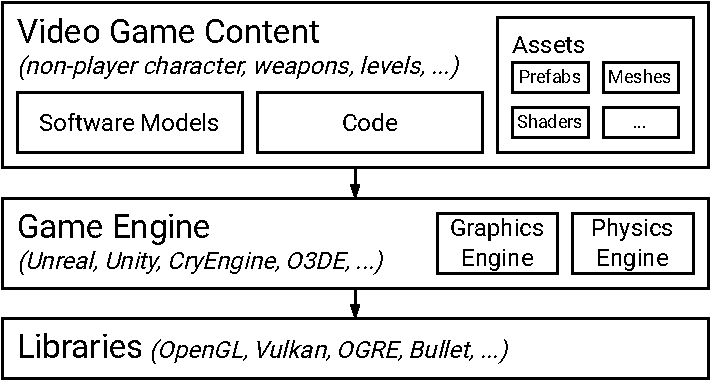
\includegraphics[width=0.45\textwidth]{Figures/fig_bg_OverviewArtifactsVG.pdf}
    \caption{Overview of video game artifacts.}
    \label{fig:architecture}
\end{figure}

\subsection{\CaseStudy{}}

The research presented in this paper is framed within the context of a commercial video game case study, \CaseStudy{}. In particular, our evaluation uses the bosses of the video game to evaluate the approach. Each level of \CaseStudy{} consists of a three-dimensional space where a player-controlled spaceship has to fly from a starting point to a target destination, reaching the goal before being destroyed. The gameplay experience involves exploring floating structures, avoiding asteroids, and finding items along the route, while basic enemies try to damage the spaceship by firing projectiles. If the player manages to reach the destination, the final boss corresponding to that level appears and must be defeated in order to complete the level. 

Bosses can be built either using C++ code or software models. The top part of Figure~\ref{fig:scenario} depicts a boss fight scenario where the player-controlled ship (item A in the figure) is battling The Serpent (item B in the figure), which is the final boss that must defeated in order to complete Level 1. The bottom part of the figure illustrates the two possible development approaches for the boss.

\begin{figure}[h]
    \centering
    \includegraphics[width=\columnwidth]{Figures/MM_Scenario.pdf}
    \caption{Model-Driven Development vs. Code-Centric Development in the context of \CaseStudy{}}
    \label{fig:scenario}
\end{figure}

Even though Figure~\ref{fig:scenario} shows excerpts of the implementation of The Serpent both in the form of software models and code, it is not necessary to implement the two simultaneously. Although developers can mix both technologies, developing different parts of the boss using one or the other indistinctly, they are also free to implement the content using software models exclusively or to do so purely via code. However, the heterogeneous nature of video game development teams - comprised majorly of programmers~\cite{devNation}, but also counting game designers, artists, UI designers, and QA engineers within their ranks - possibly favours the use of software models over code, since the higher abstraction level of the former (combined with their detachment from more technical implementation details) empowers less tech-focused roles to embrace a more active participation in development tasks. Furthermore, an experiment~\cite{domingo2020evaluating} confirmed that video game developers make fewer mistakes and are more efficient when working with the models than with the code.

Within the context of \CaseStudy{}, the elements of the game are created through software models, and more specifically, through the Shooter Definition Model Language (SDML). SDML is a DSL model for the video game domain that defines aspects that are included in video game entities: the anatomical structure (including their components, physical properties, and connections); the amount and distribution of vulnerable parts, weapons, and defenses; and the movement behaviours associated to the whole body or its parts. SDML has concepts such as hulls, links, weak points, weapons, and AI components, and allows for the development of any game element, such as bosses, enemies, or environmental elements. The models are created using SDML and interpreted at runtime to generate the corresponding game entities. In other words, software models created using SDML are translated into C++ objects at runtime using an interpreter integrated into the game engine~\cite{blasco2021evolutionary}. More information on the SDML model can be found in the following video presentation: \url{https://youtu.be/Vp3Zt4qXkoY}.


\section{Our \ApproachName{} Approach} 
\label{sec:Approach}

This section explains how our \ApproachName{} approach makes use of evolutionary computation to transplant organs within video games content. We first present an overview of our approach and subsequently provide the details of the approach. To help the reader, we provide along with the approach explanation an example of transplantation of content within a simplified version of \sq{bosses} of the video game \CaseStudy{}.

Fig.~\ref{fig:approach} shows an overview of our approach.
At the top left of the figure we show the input to our approach, which are the organ to be transplanted from the donor and the host where the organ will be transplanted. Afterwards, \ApproachName{} detects the points of the organ that allows the transplantation and the points where the organ can be inserted into the host. To initialize the population of the evolutionary algorithm, the organ is cloned and transplanted in a random point. Genetic operations generate potential solutions for transplantation, while the objective function asses the quality of these solutions. This process of generating and assessing is repeated until a specific stop condition is met. When the evolutionary algorithm finish the execution we obtain a ranked list by the objective function of the best transplantation between organ and host.

In video games, software models are popular (compared to classic software) possibly because they facilitate the participation of non-programmers (e.g. artists) in the development process. Therefore, our \ApproachName{} approach is designed to work with models. Although we illustrate the running example with the SDML models of the case study, our approach is generic and can be used with other modelling languages because it exploits the idea of boundaries between model elements.
Next, we describe each step of \ApproachName{} in the following subsections.

\begin{figure}[h]
    \centering
    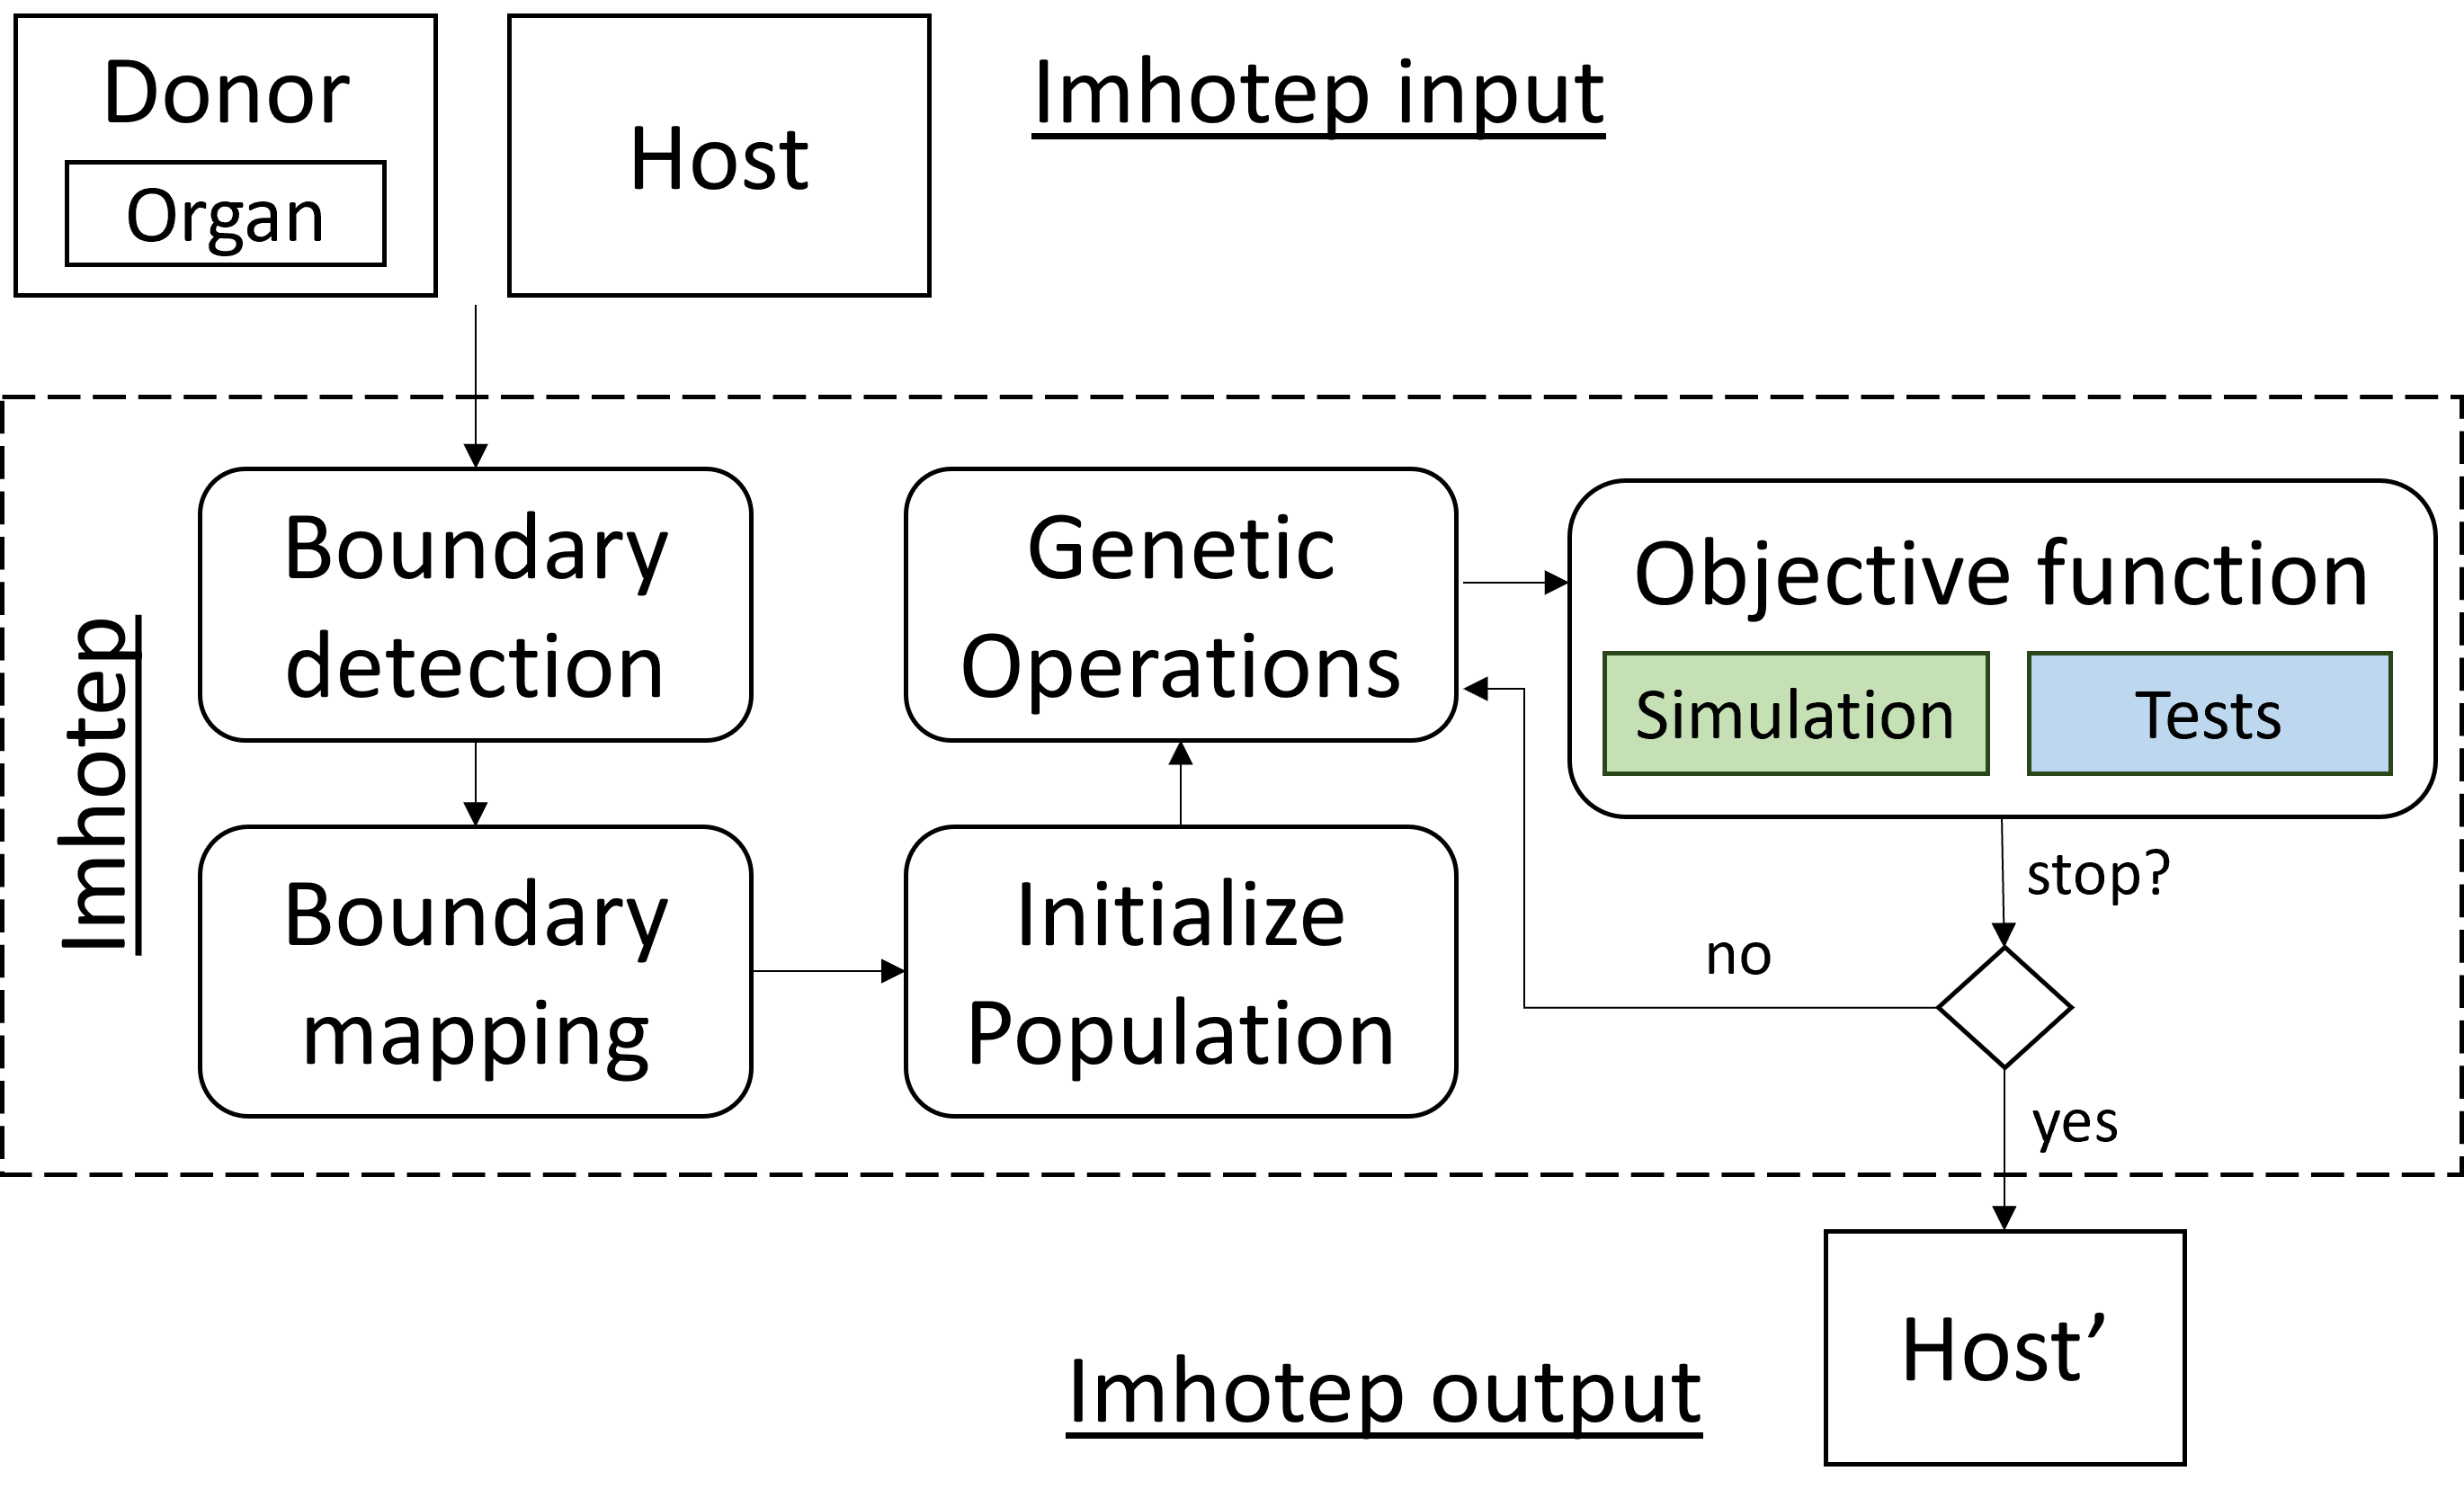
\includegraphics[width=0.45\textwidth]{Figures/overview.png}
    \caption{Overview of our \ApproachName{} approach.}
    \label{fig:approach}
\end{figure}


\subsection{Input selection}

\ApproachName{} requires the developers to identify a source model content (donor) with the organ that will be transplanted, and a target model content (host). %The models used in \ApproachName{} are models based on SDML as explained in the background section (\ref{sec:Background}). The donor and host from the example are a simplified version of the donor and host used in the evaluation, which we think they will help to understand the approach.
In our running example we present a simplified version of the metamodel, and the corresponding concrete syntax of the model (see Fig.~\ref{fig:metamodel+syntax}) from the video game \CaseStudy{}. 
\sq{Hulls} serve as the structural framework that define the anatomical composition of the models. For example, the boss presented on Fig.~\ref{fig:scenario} (identified as \sq{B}) has its body built by hulls.
\sq{Weak points} points are conceptual elements that possess the vulnerability to be harmed.
\sq{Weapons} are tangible items capable of causing harm through direct contact, such as discharging projectiles like bullets.
Hulls, weak points, and weapons are attached between them through \sq{Links}.
%We use a graphical representation to help the comprehension of the reader, however the original metamodel does not work with a graphical model representation as it is not a requirement on every metamodel. The type of model will depend on the metamodel and models that developers decide on.

\begin{figure}[h]
    \centering
    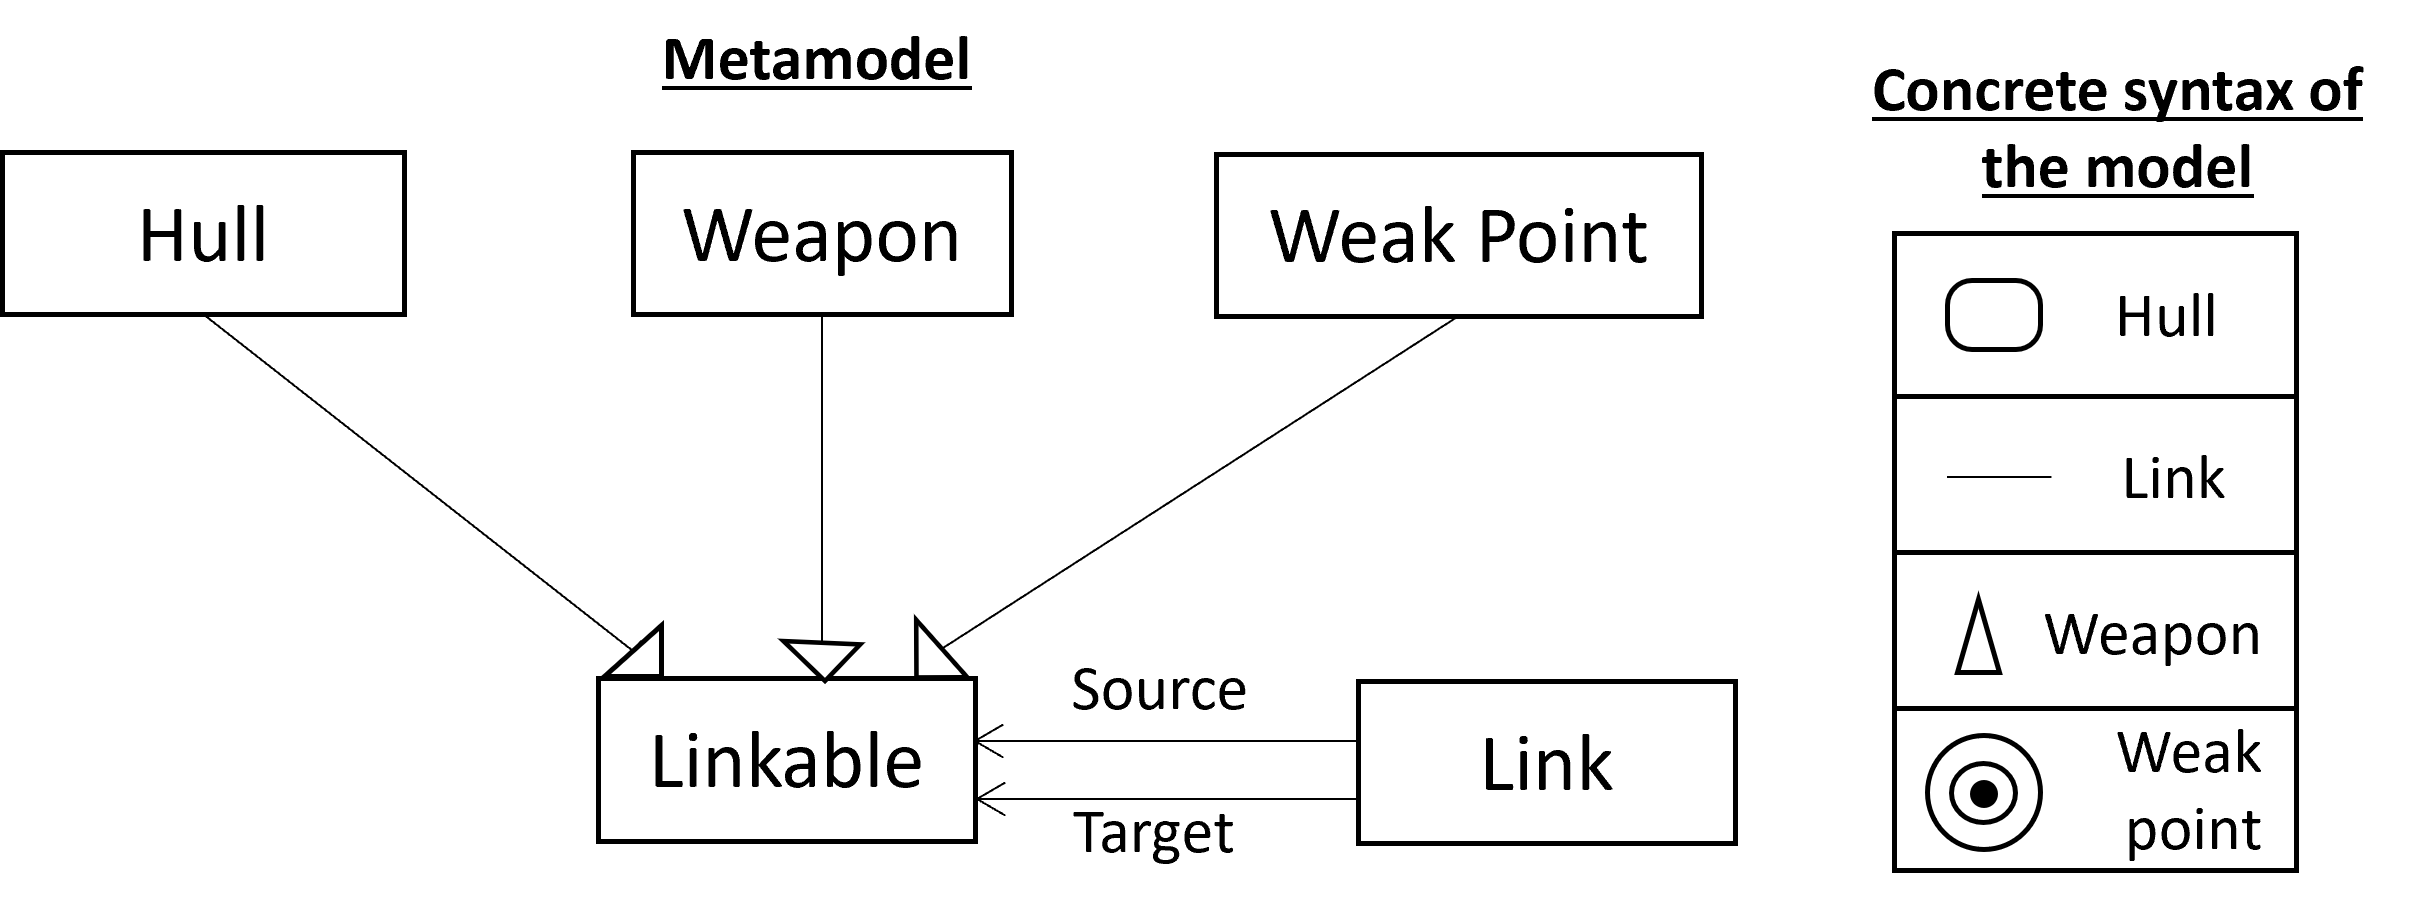
\includegraphics[width=0.35\textwidth]{Figures/metamodel+syntax.png}
    \caption{Simplified metamodel with the corresponding concrete syntax of the model.}
    \label{fig:metamodel+syntax}
\end{figure}

In the running example, the source donor model is a simplified version of an original \sq{boss} from \CaseStudy{}, called \sq{Serpent}. Fig.~\ref{fig:donor} shows the graphical representation of the donor model, differentiating each element of the model with a letter from A to S. It also shows with dashed lines the elements selected as organ (the elements H, I, J, K, N, O, P, Q).
This simplified example is inspired by the boss shown in Fig.~\ref{fig:scenario} with letter B. In the running example, the host is a model of a regular enemy that could appear in \CaseStudy{}. Fig.~\ref{fig:host} shows the graphical representation of the host model.

\begin{figure}[h]
    \centering
    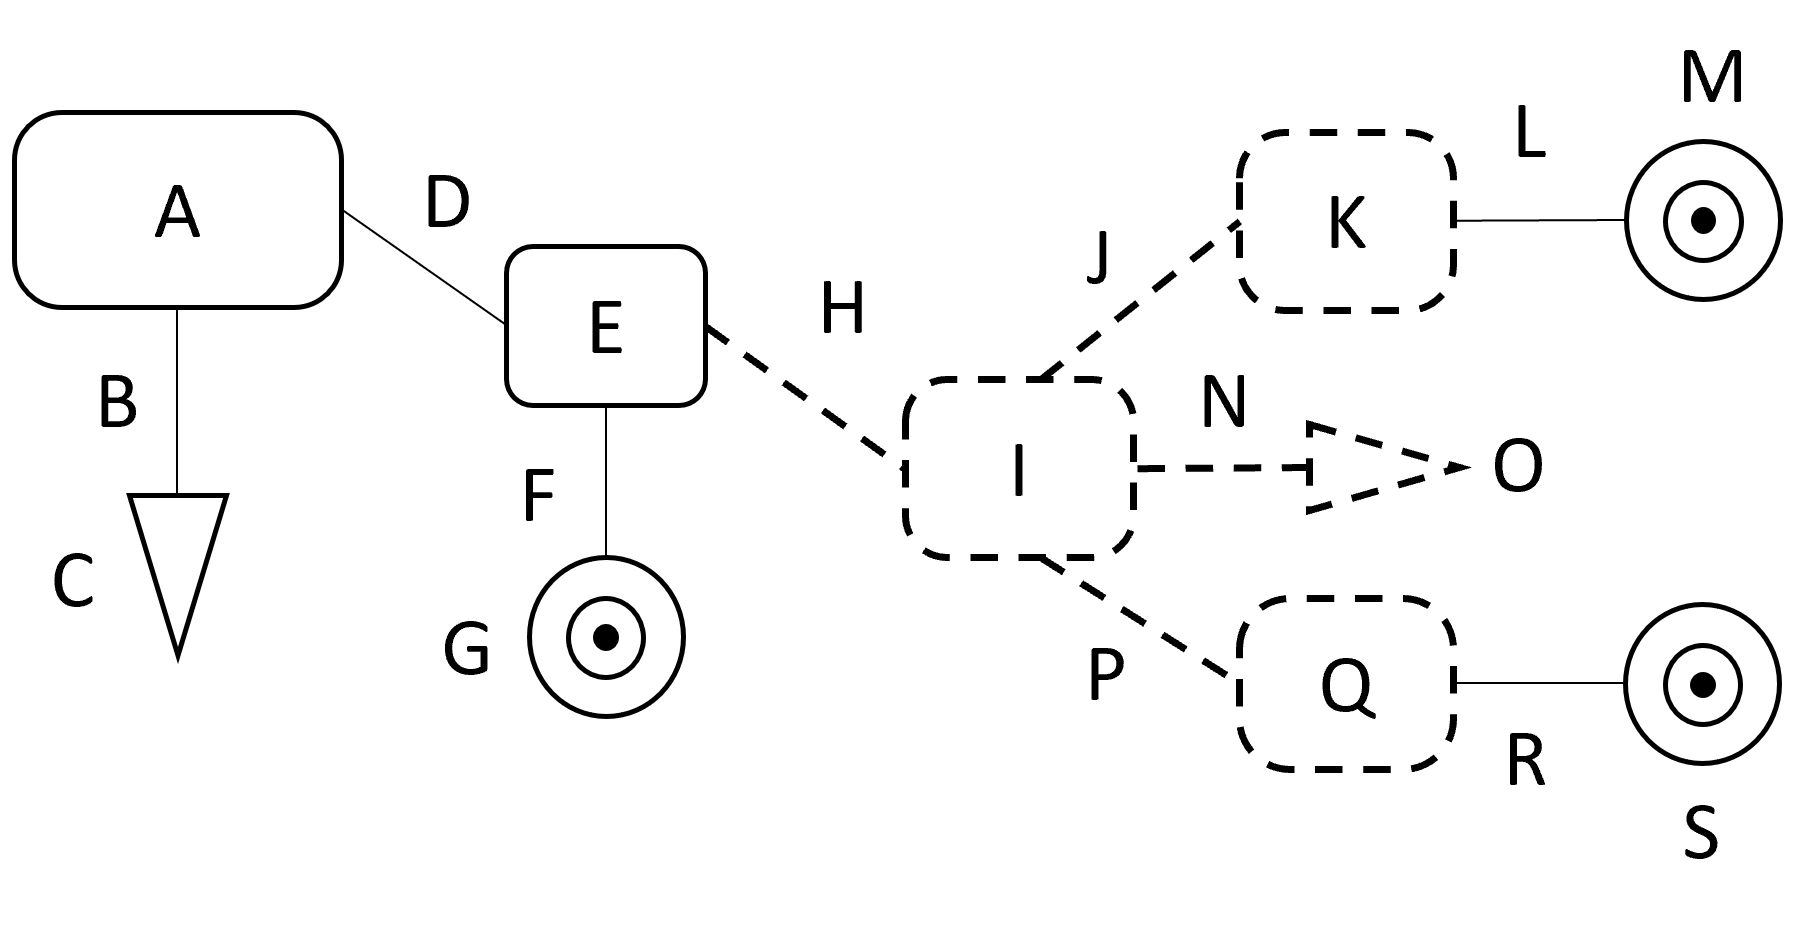
\includegraphics[width=0.35\textwidth]{Figures/donor+organ.png}
    \caption{Donor model with organ selection in dashed lines.}
    \label{fig:donor}
\end{figure}

\begin{figure}[h]
    \centering
    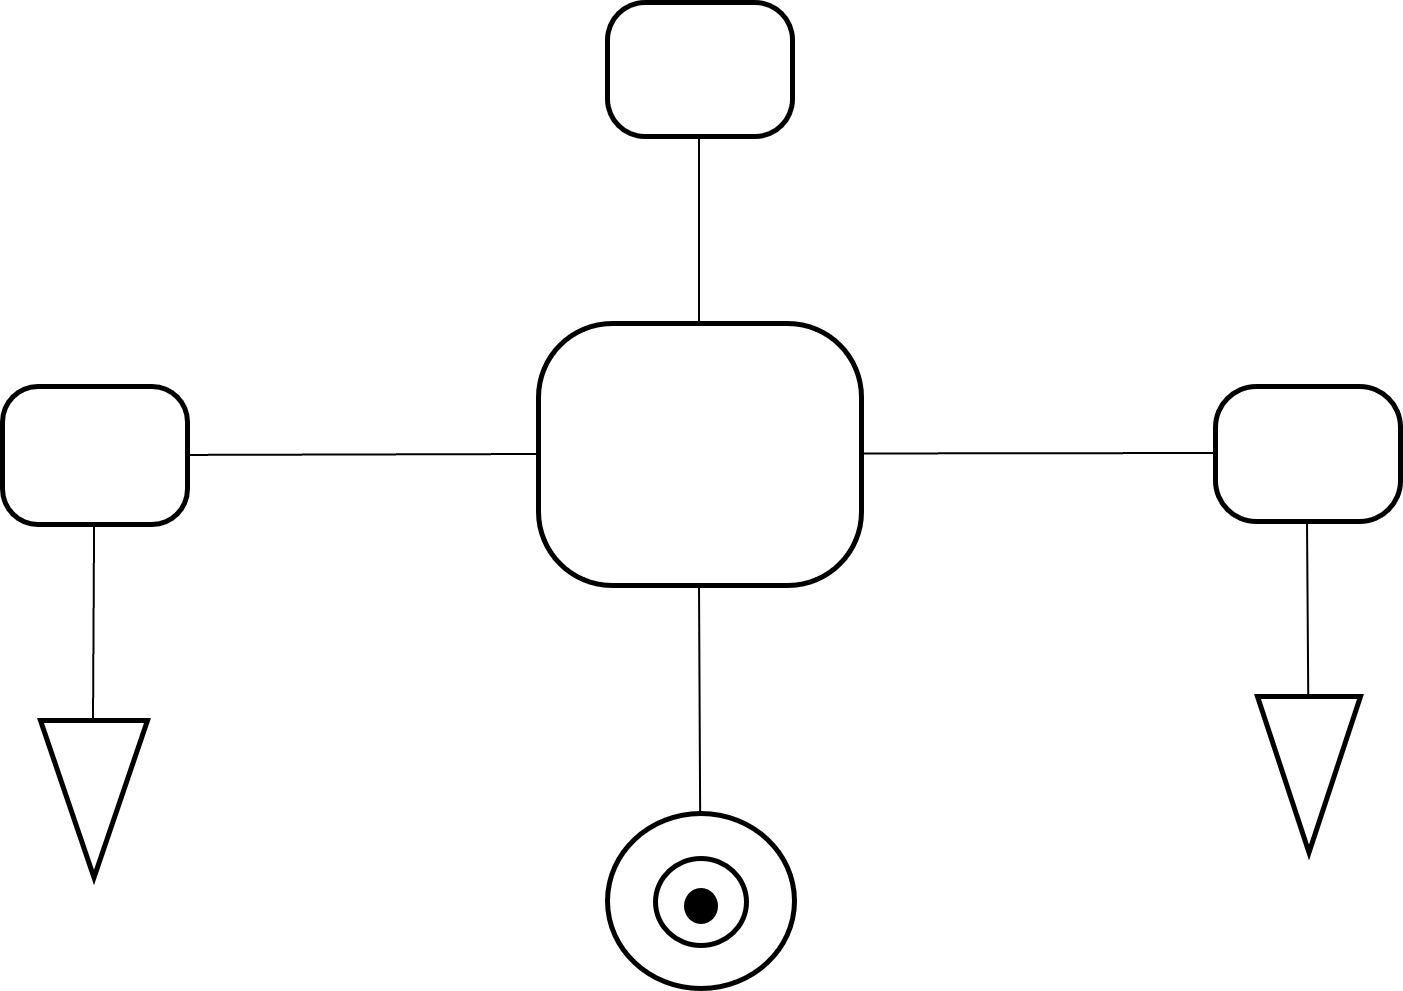
\includegraphics[width=0.2\textwidth]{Figures/host.png}
    \caption{Host}
    \label{fig:host}
\end{figure}

\subsection{Boundary detection}

To transplant an organ into a host we need to find a way to connect them. To do that we use the boundaries between the model elements of the organ and the host. A boundary is a connection point capable of connecting two distinct model elements within a model. The connection is restricted by the rules of the metamodel. In the simplified example in Fig.~\ref{fig:metamodel+syntax}, the Source and Target meta-relationships are the boundaries between the model elements of the models conforming to that metamodel. In other metamodel languages, there will be other meta-relationships with other names that will be the boundaries.

Imhotep automatically identifies the boundaries of the selected organ, and all the boundaries of the host. In the running example, the boundaries of the organ are the connection points between donor and host. The elements that connect with the rest of the donor are H, K, and Q. Fig.~\ref{fig:org_bound} shows the donor, the organ, and the boundaries (boundaries are represented by a circle crossed). The boundaries of the organ are as follows: b11 for the H element; b16 for the K element, and b25 for the Q element.

\begin{figure}[h]
    \centering
    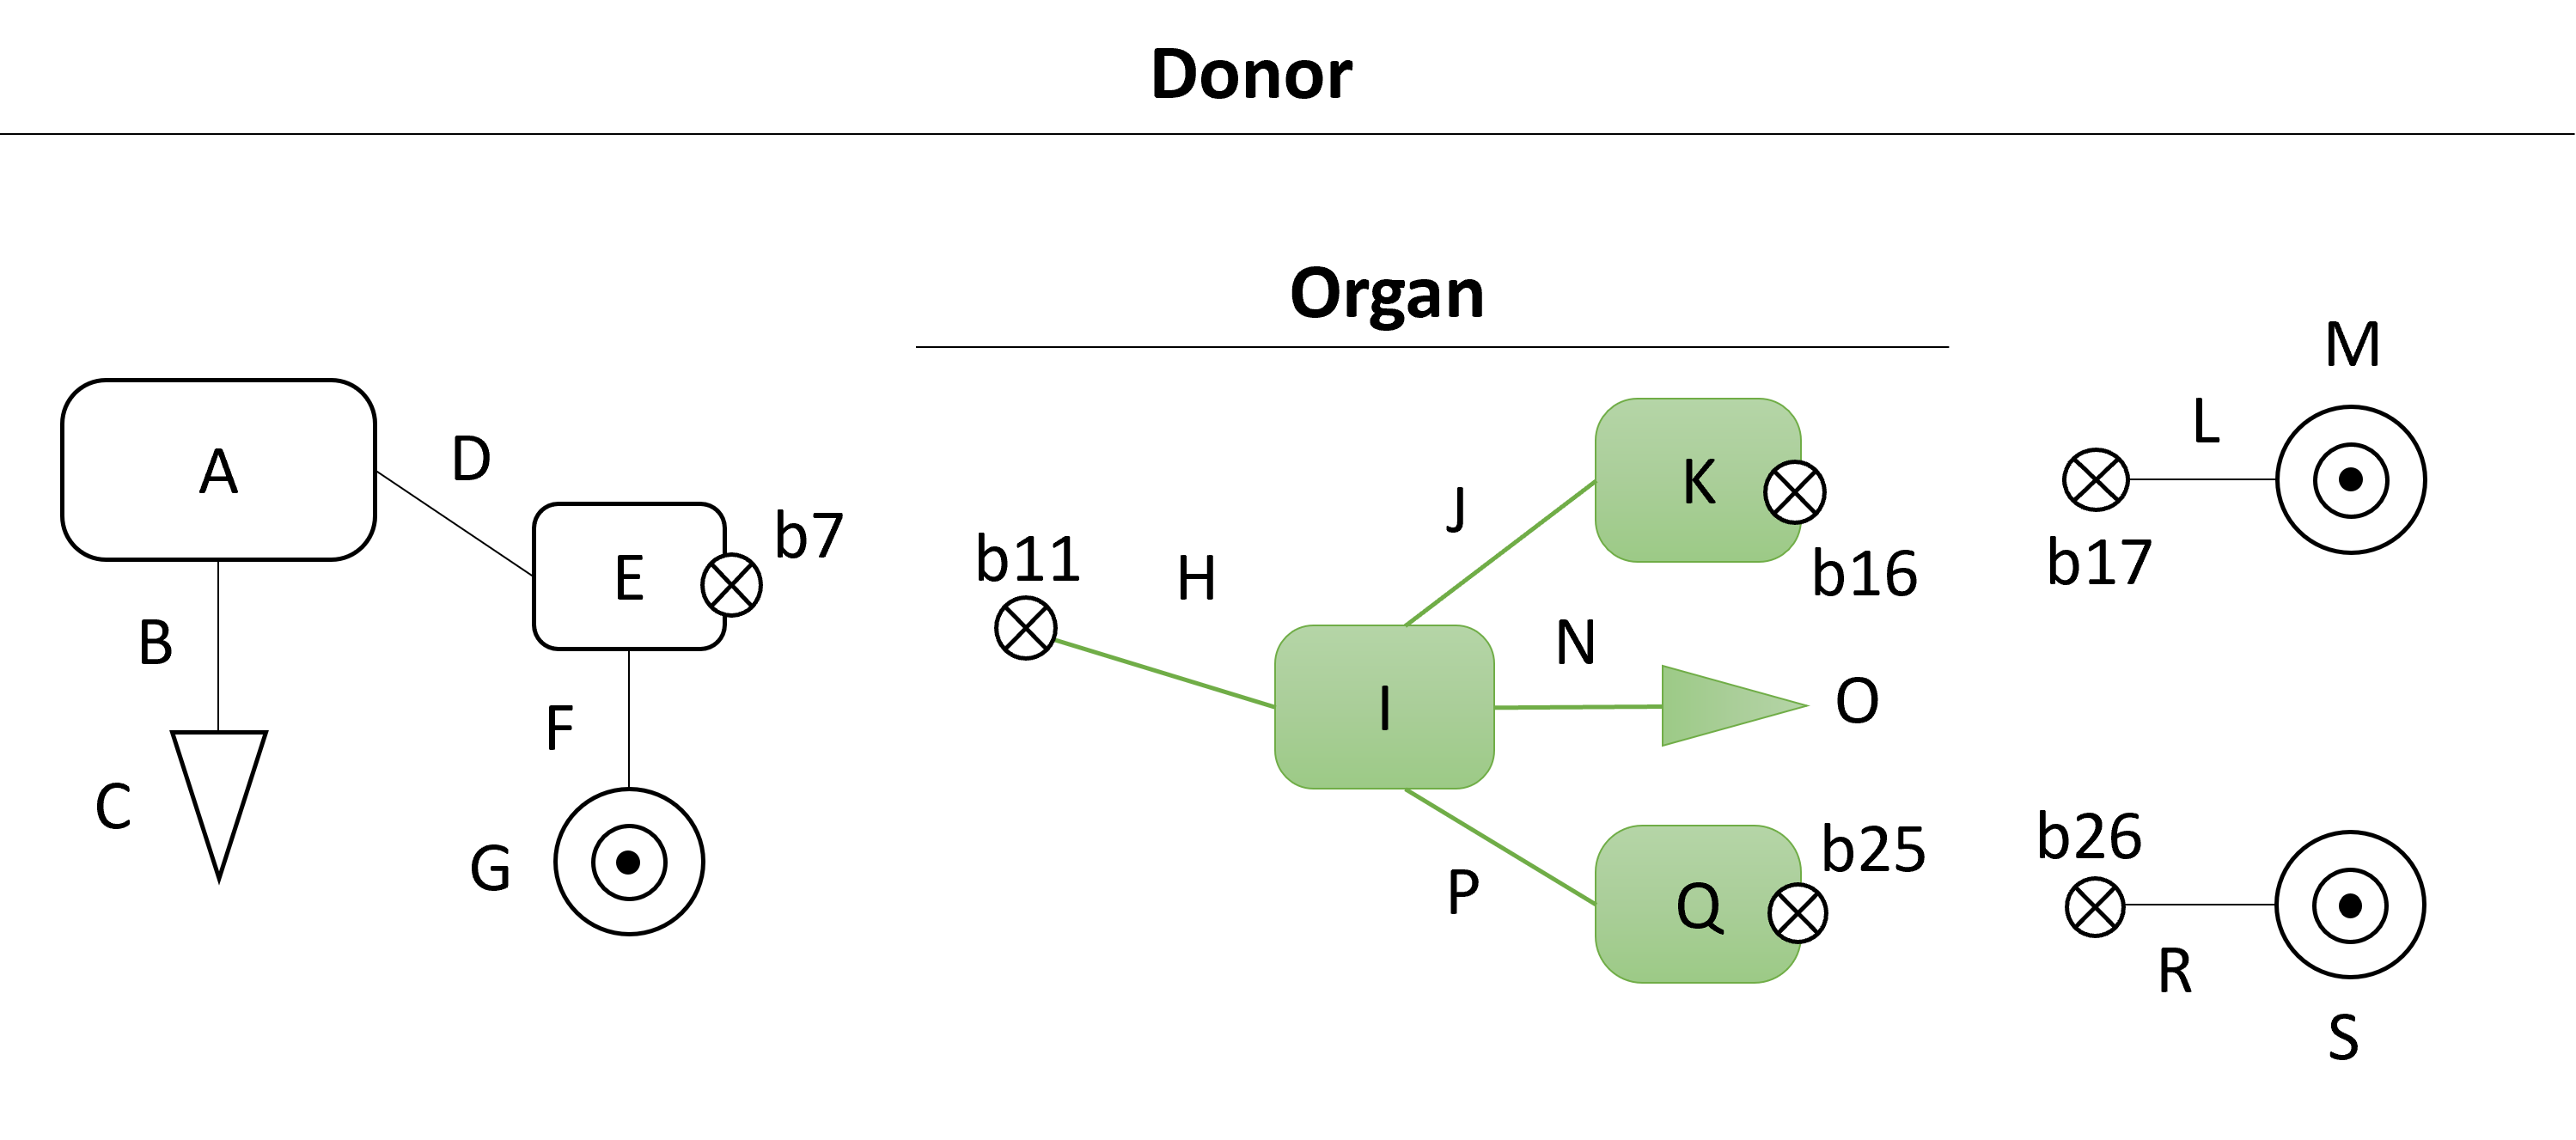
\includegraphics[width=0.45\textwidth]{Figures/donor+organ_boundaries.png}
    \caption{Donor model boundaries. The boundary is represented by a circle crossed.}
    \label{fig:org_bound}
\end{figure}

On the other hand, the boundaries of the host are all the points where its model elements connect. Figure~\ref{fig:host_bound} shows all the boundaries of the host of the running example. The host has a total of 19 boundaries identified by a tag from ba to bs.

\begin{figure}[h]
    \centering
    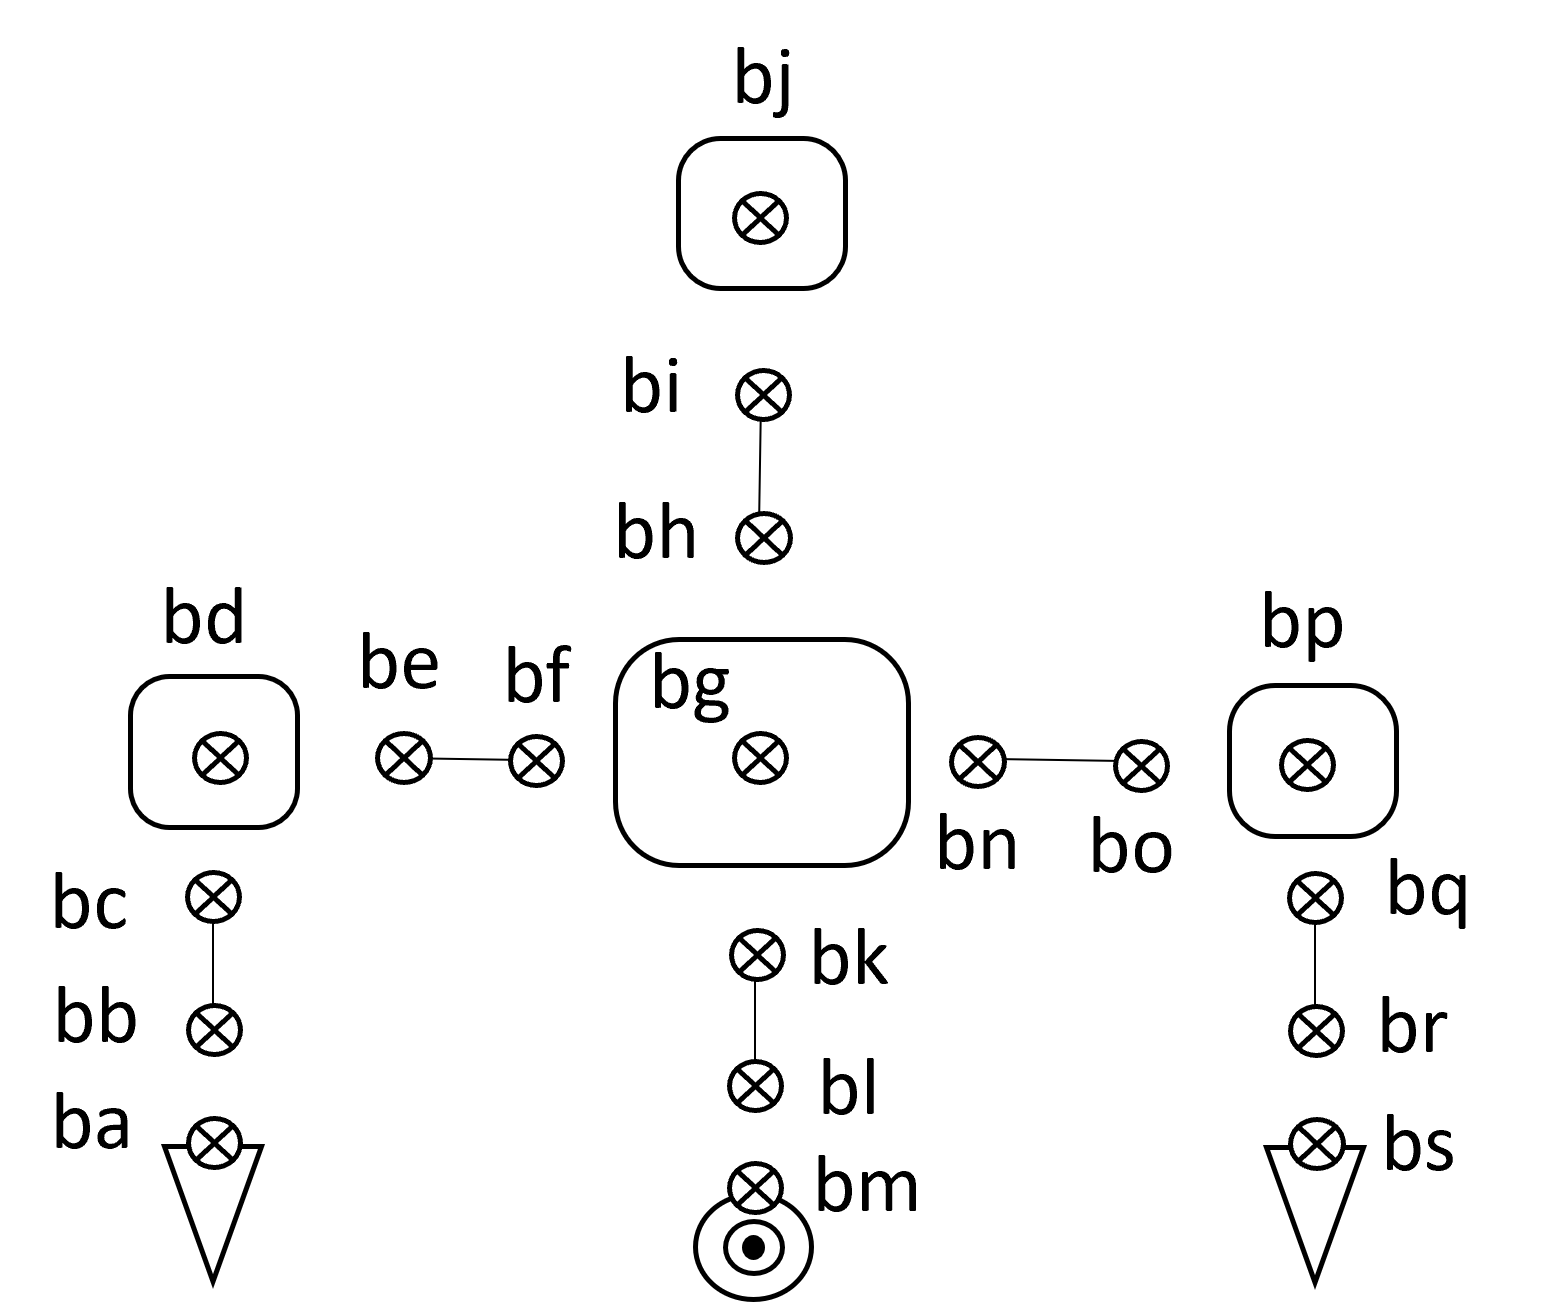
\includegraphics[width=0.35\textwidth]{Figures/host_boundaries.png}
    \caption{Host model boundaries. The boundary is represented by a circle crossed.}
    \label{fig:host_bound}
\end{figure}

\subsection{Boundary mapping}

In the boundary mapping step, \ApproachName{} determines the mapping between the boundaries of the organ and the host. For each boundary in the organ, Imhotep considers all compatible boundaries of the host, including the possibility of not connecting the boundary to the host boundaries. The boundary compatibility is determined by the metamodel.

Table~\ref{tab:boundaries} shows a boundary mapping between the organ and the host of the running example. The boundary b11 is a boundary from a \sq{Link} from the model and according to the metamodel it can connect to any \sq{Hull}, \sq{Weapon}, \sq{Weak Point}. The boundaries b16 and b25 are both \sq{Hulls} and they can connect with any \sq{Link}.

\begin{table}[h]
\centering
\resizebox{0.35\textwidth}{!}{
\begin{tabular}{|c|ll|}
\hline
{Organ boundaries} & \multicolumn{2}{c|}{{ \begin{tabular}[c]{@{}c@{}}Host \\      boundaries\end{tabular}}} \\ \hline
& \multicolumn{1}{c|}{ba} & \multicolumn{1}{c|}{bm} \\ \cline{2-3} 
& \multicolumn{1}{c|}{bd} & \multicolumn{1}{c|}{bp} \\ \cline{2-3} 
& \multicolumn{1}{c|}{bg} & \multicolumn{1}{c|}{bs} \\ \cline{2-3} 
\multirow{-4}{*}{b11} 
& \multicolumn{1}{c|}{bj} & \multicolumn{1}{c|}{Not connected} \\ \hline
& \multicolumn{1}{c|}{bb} & \multicolumn{1}{c|}{bc} \\ \cline{2-3} 
& \multicolumn{1}{c|}{be} & \multicolumn{1}{c|}{bf} \\ \cline{2-3} 
& \multicolumn{1}{c|}{bh} & \multicolumn{1}{c|}{bi} \\ \cline{2-3} 
& \multicolumn{1}{c|}{bk} & \multicolumn{1}{c|}{bl} \\ \cline{2-3} 
& \multicolumn{1}{c|}{bn} & \multicolumn{1}{c|}{bo} \\ \cline{2-3} 
\multirow{-6}{*}{\begin{tabular}[c]{@{}c@{}}b16\\    \\ b25\end{tabular}} 
& \multicolumn{2}{c|}{Not connected} \\ \hline
\end{tabular}}
\caption{Mapping  of compatible boundaries between organ and host.}
\label{tab:boundaries}
\end{table}

\subsection{Initialize population}

In evolutionary algorithms a population is a collection of possible solutions for a problem.
The encoding is the problem representation that an algorithm is capable to understand. 

In our work, the encoding requires a binary vector that represents the organ in the donor, and the boundary mapping (see Fig.~\ref{fig:encoding}). In the binary vector, each element from the model is a position from the vector. If a position in the vector has a \sq{1}, it means that the element from the model is part of the organ. On the other hand, each boundary from the organ gets assigned a compatible boundary from the host.
%In our work, each individual represents a software model from the game. We use a similar encoding version of Blasco \etal~\cite{blasco2021evolutionary} that has been adapted to work with transplantations. The size of the encoding in the previous work was 64 and in this work its size is of 150.
The initial population of Imhotep contains individuals composed by the host and the organ placed in a random position (a random mapping between the organ boundaries and the compatible organ boundaries).

\begin{figure}[h]
    \centering
    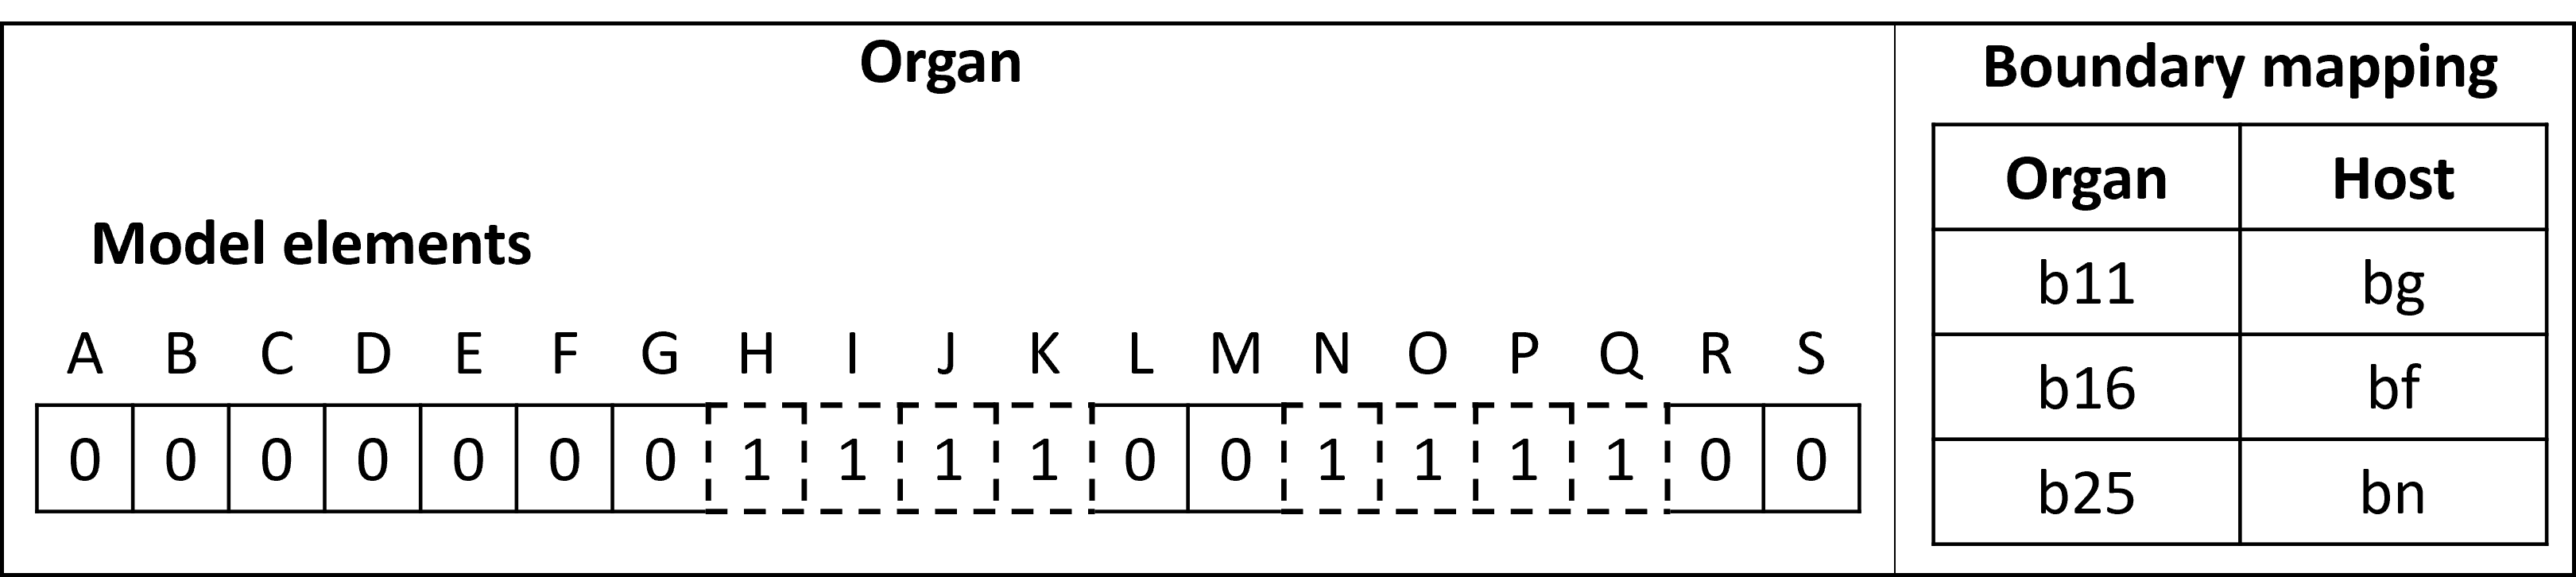
\includegraphics[width=0.48\textwidth]{Figures/encoding.png}
    \caption{Example of encoding.}
    \label{fig:encoding}
\end{figure}

\subsection{Genetic Operators}

Imhotep has genetic operations (selection, crossover, and mutation) to generate new individuals of the population. To select the individuals, we use the ranking selection, which ranks the population by the objective function and takes the top individuals in the current population.

We use a single, random, cut-point crossover. It starts by selecting and splitting two parent solutions at random. When two parent individuals are selected, a random cut point is determined to split them into two sub-vectors.
Then, the crossover creates two child solutions by putting the first part of the first parent with the second part of the second parent for the first child and putting the first part of the second parent with the second part of the first parent for the second child.
Finally, the new individual has a probability to mutate any value of the encoding. 

Fig.~\ref{fig:candidates} shows example of new individuals that could results from the running example. For simplicity, these individuals have unaltered organs but illustrate different boundary mappings between organ and host.

\begin{figure}[h]
    \centering
    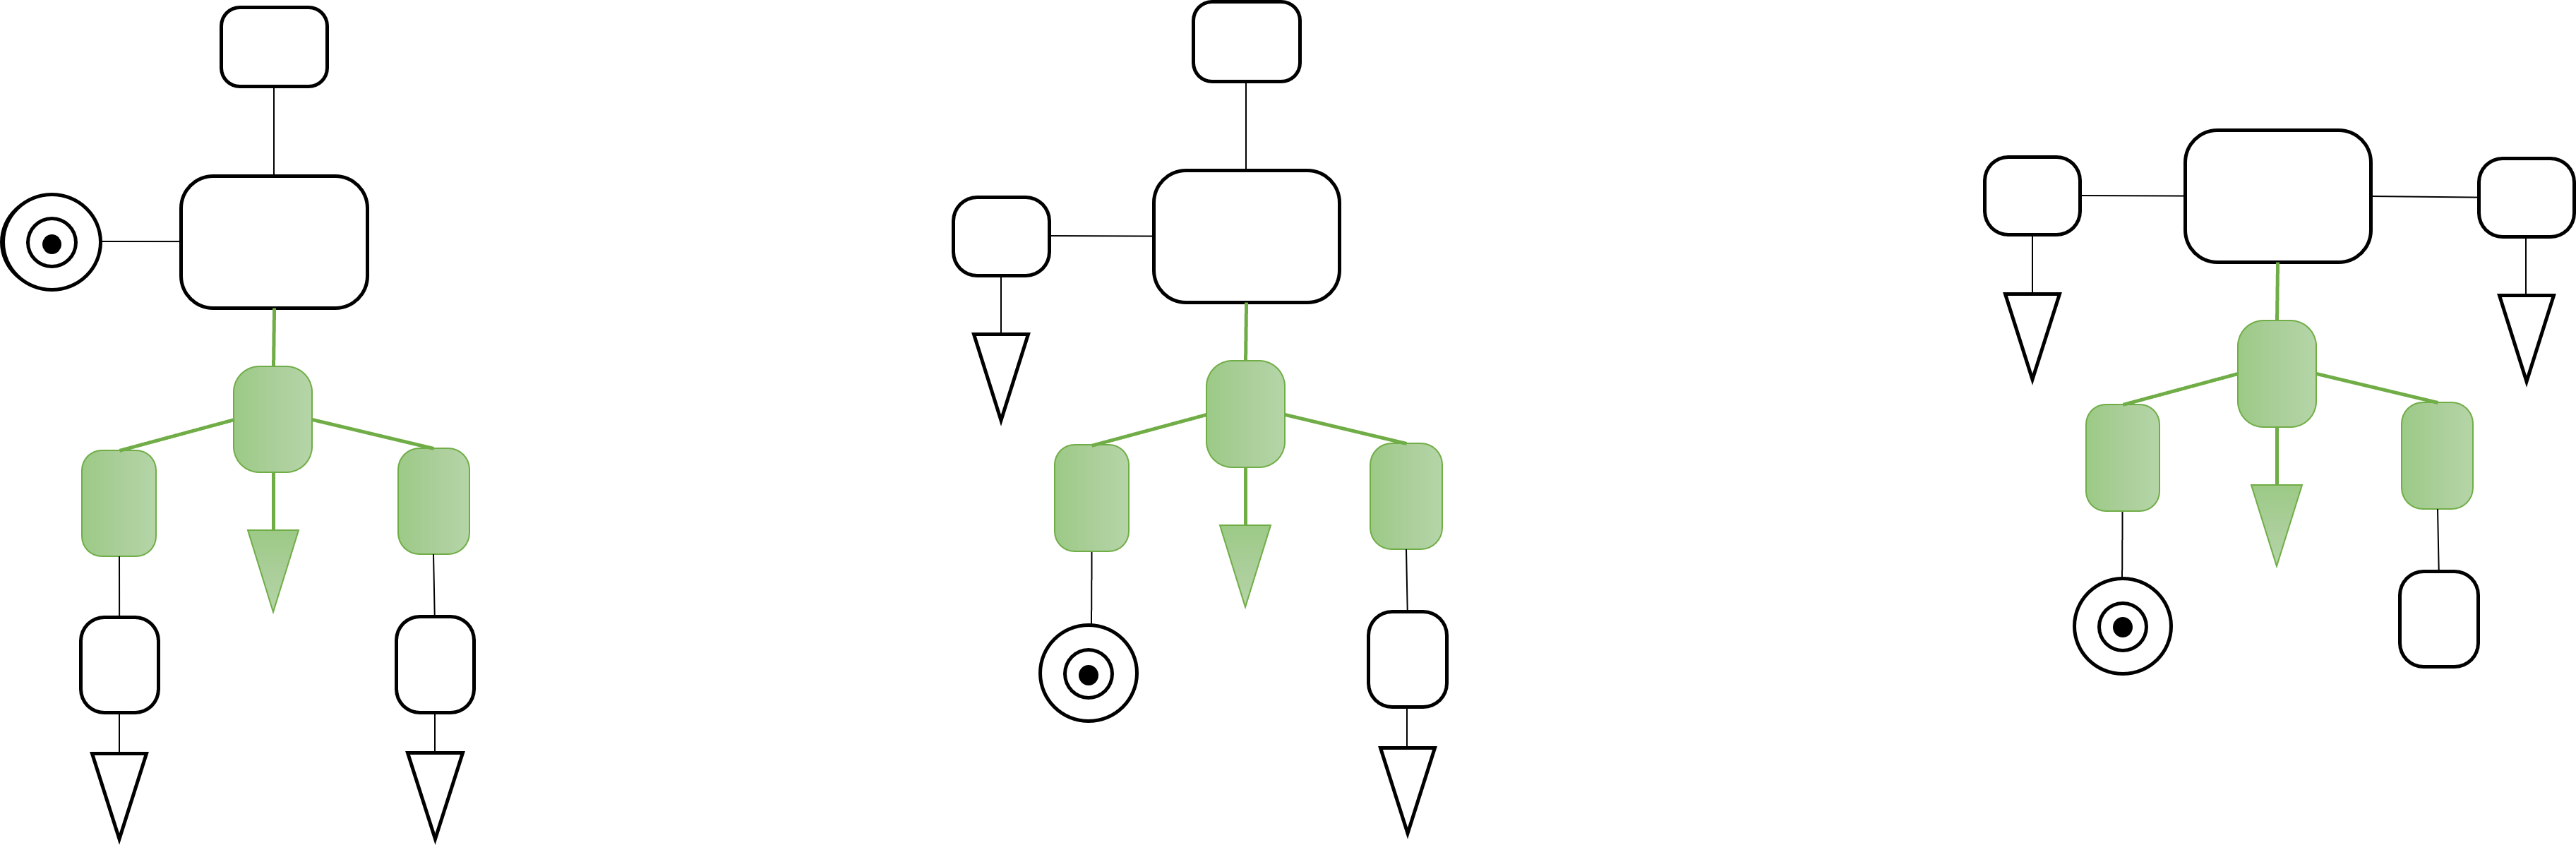
\includegraphics[width=0.45\textwidth]{Figures/candidates.png}
    \caption{Example of individuals.}
    \label{fig:candidates}
\end{figure}

\subsection{Objective function}

Our work proposes to harness video games' NPCs to run simulations that provide data to assess the transplantations. The first thing that differentiates video games from traditional software is that the basic requirement of video games is \sq{fun}. \sq{Fun} is an abstract concept and the developers are in charge of interpreting it. In fact, different developers may have different interpretations. For some game developers, \sq{fun} is achieved with a difficult game that is very rewarding when progress is made (e.g., Dark Souls). While for other developers, \sq{fun} is achieved by effortlessly killing enemies (e.g., Dynasty Warriors). Therefore, we argue that the developer intent is key for content generation.

Specifically, we propose to introduce the generated content (each individual in the population) into a simulation of the video game. The simulation produces a data trace of the events that have occurred. Using the data from the trace, we can check how well aligned are the events with the intention of the developers. In the running example, the simulation is a duel between a spaceship and a boss. The simulation generates data about the duel, such as the damage inflicted. The intention of the developers may be that the duel ends with the victory of the spaceship with a remaining life of less than 10\%.

Our proposal does not require ad hoc development of simulations. We propose that the simulations leverage mainly the NPCs (but also more video game elements, such as scenarios or items like weapons or powerups). NPCs are naturally developed during the development process of a video game. In other words, NPCs are integral components of  most video game genres such as First-Person Shooter (FPS), Real-Time Strategy (RTS), our racing games. We aim two goals with the aforementioned. On the one hand, it makes the use of simulations cheaper, i.e. it does not involve additional development costs, and secondly, it facilitates fidelity to the video game compared to ad hoc development. In the running example, during the simulation, the generated content is the boss, who can be accompanied by more NPCs acting as secondary enemies. Additionally, the spaceship that confronts the boss is a NPC representing an allied ship. Finally, the scenario, and items such as weapons or powerups also belong to the game itself.

In this work, the Simulation-based variant of \ApproachName{} assesses the transplants through a simulation of a game battle between the boss (Host') and a NPC spaceship. The information retrieved from the simulation is the data that the developers regard as relevant, using their domain knowledge. Hence, our approach takes into account  the percentage of simulated player victories ($F_{Victory}$) and the percentage of simulated player health left once the player wins a duel ($F_{Health}$).
The calculation of $F_{Victory}$ and $F_{Health}$ is performed in the same
way as Blasco \etal~\cite{blasco2021evolutionary}:

$F_{Victory}$ is calculated as the difference between the number of human player victories ($V_{P}$) and the optimal number of victories (33\%, according to the developers of \CaseStudy{} and their criteria) ($V_{Optimal}$):
\begin{equation}
F_{Victory} = 1 -\frac{\mid V_{Optimal} - V_{P} \mid}{ V_{Optimal}}
\end{equation}

$F_{Health}$, which refers to completed duels that end in spaceship victories, is the average difference between the spaceship's health percentage once the duel is over ($\Theta_{P}$) and the optimal health level that the spaceship should have at that point ($\Theta_{Optimal}$, 20\%, according to the developers):
\begin{equation}
F_{Health} = 1 - \frac{\sum\limits_{d=1}^{V_{P}}\frac{\mid \Theta_{Optimal} - \Theta_{P} \mid}{ \Theta_{Optimal}}}{V_{P}}
\end{equation}

$F_{Overall}$ is an average fitness value for a boss model that includes the fitness criteria described above. FOverall also includes a validation part. The validation part is to avoid models with inconsistencies. The validity of the models is performed by a run-time interpreter that is part of the game. When the model is stated as non-valid the value of Validity will be 0. $F_{Overall}$ can assume a value in [0, 1] which is used to assess a boss model when our \ApproachName{} approach is applied to the \CaseStudy{} case study.

\begin{equation}
F_{Overall} = min( Validity, \frac{\sum\limits_{i=1}^{N}F_{i}}{N} )
\end{equation}


% The objective function in \ApproachName{} assesses the quality of each individual as a model. First, as done in previous work that use \CaseStudy{}~\cite{blasco2021evolutionary}, the models pass through a validation process followed by a quantitative measurement. In our work we assess quantitatively the objective function by two means: Test-based and Simulation-based objective functions. We use two different objective functions due to the differences in the the state-of-the-art of software transplantation and PCG. The state-of-the-art in software transplantation mainly work with Test-based objective function, while the state-of-the-art in NPCs PCG work with Simulation-based objective function.

% The validation step before the Test-based or Simulation objective function is a requirement that \CaseStudy{} integrates in the game to avoid models with inconsistent data. The validity of the models is performed by a run-time interpreter that is part of the game. When the model is stated as non-valid the value of the objective function will be 0.0.

% The models that pass the validation process will then be assess by the Test-based and Simulation-based objective functions.
% For the Test-based objective function we ask the developers to provide the set of tests that they consider relevant to our work. The developers from \CaseStudy{} provided us with a total of 243 tests selected based on their domain knowledge. The objective value will be retrieved when each individual pass through the 243 tests, normalized in a scale of [0, 1]. An individual which passes the 243 tests will obtain 1.0, on the contrary if it does not pass any test it will obtain 0.0.

% On the other hand, the Simulation-based objective function as in Blasco \etal~\cite{blasco2021evolutionary} simulates an in game battle between the boss and a player. The information retrieved from the simulation is the data that the developers regard as relevant, using their domain knowledge. Hence, our approach takes into account the percentage of simulated player victories ($F_{Victory}$) and the percentage of simulated player health left once the player wins a duel ($F_{Health}$).
% The calculation of $F_{Victory}$ and $F_{Health}$ is performed in the same
% way as Blasco \etal~\cite{blasco2021evolutionary}:

% $F_{Victory}$ is calculated as the difference between the number of human player victories ($V_{P}$) and the optimal number of victories (33\%, according to the developers of \CaseStudy{} and their criteria) ($V_{Optimal}$):
% \begin{equation}
% F_{Victory} = 1 -\frac{\mid V_{Optimal} - V_{P} \mid}{ V_{Optimal}}
% \end{equation}

% $F_{Health}$, which refers to completed duels that end in human player victories, is the average difference between the human player's health percentage once the duel is over ($\Theta_{P}$) and the optimal health level that the player should have at that point ($\Theta_{Optimal}$, 20\%, according to the developers):
% \begin{equation}
% F_{Health} = 1 - \frac{\sum\limits_{d=1}^{V_{P}}\frac{\mid \Theta_{Optimal} - \Theta_{P} \mid}{ \Theta_{Optimal}}}{V_{P}}
% \end{equation}

% $F_{Overall}$ is an average fitness value for a boss model that includes the fitness criteria described above. $F_{Overall}$ can assume a value in [0, 1] which is used to assess a boss model when our \ApproachName{} approach is applied to the \CaseStudy{} case study.

% \begin{equation}
% F_{Overall} = min( Validity, \frac{\sum\limits_{i=1}^{N}F_{i}}{N} )
% \end{equation}

\section{Experimental Design} 
\label{sec:Evaluation}

In this section we explain how we empirically evaluate our proposal for automated transplantation in video games through \ApproachName{}. Through this section, we present the research questions that we aim to answer, the evaluation process, and the implementation details.

\subsection{Research Questions}

\simhotep{} propose a new angle for PCG, and for that reason we want to compare it to the established practice in the video game field in our first research question:

\textbf{RQ$_1$: }\textit{How does \simhotep{} perform with respect to the PCG baseline?}

\simhotep is also a new angle to guide the transplantation. We propose to leverage the possibilities of the vide game domain by means of simulations, so we want to compare it to the established practice (test suite to guide the transplantation) in the software transplantation field. This motivates our second research question:

\textbf{RQ$_2$: }\textit{What is the performance in terms of solution quality of \simhotep{} and \timhotep{}?}

% \textbf{RQ$_1$: }\textit{What is the performance in terms of solution quality of \ApproachName{} with the simulation-based \ApproachName{} ($S_{Imhotep}$), \ApproachName{} with the test-based \ApproachName{} ($T_{Imhotep}$), and the PCG baseline?}

% \textbf{RQ$_2$: }\textit{Is there any difference in the quality of the solution among \ApproachName{} with the simulation-based \ApproachName{}, \ApproachName{} with the test-based \ApproachName{}, and the PCG baseline?}

% \textbf{RQ$_3$: }\textit{Are the performance results obtained by \ApproachName{} with the simulation-based \ApproachName{}, \ApproachName{} with the test-based \ApproachName{}, and the PCG baseline significant?}


\subsection{Planning and execution}

Fig.~\ref{fig:evaluation} shows an overview of the evaluation. The white background part at the top shows the assets of the game itself (content) and the game development (test suite) that are used by the approaches. The grey background part in the middle shows the inputs and outputs of the three approaches (the two \ApproachName{} variants and the baseline). Finally, the white background part at the bottom shows the evaluation of the results of the approaches.

We used the work by Gallota \etal~\cite{gallotta2022evolving} as PCG baseline. Gallota \etal proposed a hybrid Evolutionary Algorithm for generating NPCs. Specifically, their approach combines an L-system with a Feasible Infeasible Two Population Evolutionary Algorithm. We choose Gallota \etal as PCG baseline because (1) this work is specific for spaceships that can play the role of bosses which is comparable to the content of the case study, and (2) it achieves the best state-of-the-art results for that content. 

In the evaluation we also include a test-based variant of \ApproachName{} (\timhotep{}). In this variant, the assessment is carried out by passing tests. The reason for including this variant is that in classic software transplantation the best results have been achieved by using the test suite for the assessment.
For the \timhotep{} we ask the developers to provide the set of tests that are relevant for the evaluation. The developers from \CaseStudy{} provided us with a total of 243 tests selected based on their domain knowledge. The objective value will be retrieved when each individual pass through the 243 tests, normalized in a scale of [0, 1]. An individual which passes the 243 tests will obtain 1.0, on the contrary if it does not pass any test it will obtain 0.0. As in the \simhotep{}, the each individual needs to pass through a validation, giving 0.0 to those that are not valid.

For the evaluation we used five different hosts (Vermis, Teuthus, Argos, Orion, and Maia), which are the full set of original bosses from the video game \CaseStudy{}. As donors, \CaseStudy{} developers considered all \CaseStudy{}'s scenarios to identify 129 organs. Each host has more than a thousand model elements. Organs have an average of 255 model elements.

Each organ was transplanted individually to each boss. Each variant of \ApproachName{} provided a total of 645 new individuals (5 hosts * 129 organs) as output, 645 new individuals from \simhotep{} and 645 individuals from \timhotep{}. In the case of the baseline (which relies on the L-system to generate the content instead of transplanting organs), to make it a fair comparison, the baseline was executed 129 times with each one of the 5 different hosts to obtain 645 new individuals. In addition, we executed 30 independent runs (to account for random variation as suggested by Arcuri and Fraser~\cite{arcuri2013parameter}). Hence, we obtain a total of 58050 independent runs (645*3*30).

To compare the solutions of the baseline and the two variants of \ApproachName{} (\simhotep{} and \timhotep{}), we rely on the concept of game quality and its automated measurement through simulated players. The results of Browne \etal demonstrated the validity of the approach which is widely accepted in the research community~\cite{browne2010evolutionary}. Therefore, we need two ingredients to run our experiment: The simulated player and the automated measurement.

The simulated player, developed by the developers of the \CaseStudy{} video game, possesses the ability to mimic human player behaviour. Our approach incorporates their algorithm, utilizing it to simulate battles between the generated bosses and the simulated player. Within these simulations, the simulated player confronts the boss, strategically targeting and destroying its weak points. Meanwhile, the boss operates in accordance with its anatomical structure, behavioural patterns, and attack/defensive dynamics, aiming to overcome the simulated player. Both entities within the simulation actively strive to emerge victorious, eschewing draws or ties, and ensuring a definitive win. The algorithm grants the simulated player the capability to employ various strategies when engaging with a boss, as it can be parameterized to define its fighting approach. The simulation parameters were provided by the developers, who analysed battles between human players and bosses to inform their decision-making.

The automated measurement is $Q_{Duration}$ which was proven to achieve good results~\cite{browne2010evolutionary}. The duration of duels between simulated players and bosses units is expected to be around a certain optimal value. For the \CaseStudy{} case study, through tests and questionnaires with players, the developers determined that concentration and engagement for an average boss reach their peak at approximately 10 minutes ($T_{Optimal}$), whereas the maximum accepted time was estimated to be 20 minutes ($2*T_{Optimal}$). Significant deviations from that reference value are good design-flaw indicators: short games are probably too easy; and duels that go on a lot longer than expected tend to make players lose interest. The criterion $Q_{Duration}$ is a measure of the average difference between the duration of each duel ($T_{d}$) and the desired, optimal duration ($T_{Optimal}$):
\begin{equation}
Q_{Duration} =  1 - \frac{\sum\limits_{d=1}^{Duels}\frac{\mid T_{Optimal} - T_{d} \mid}{T_{Optimal}}}{Duels} 
\end{equation}

\begin{figure}[h]
    \centering
    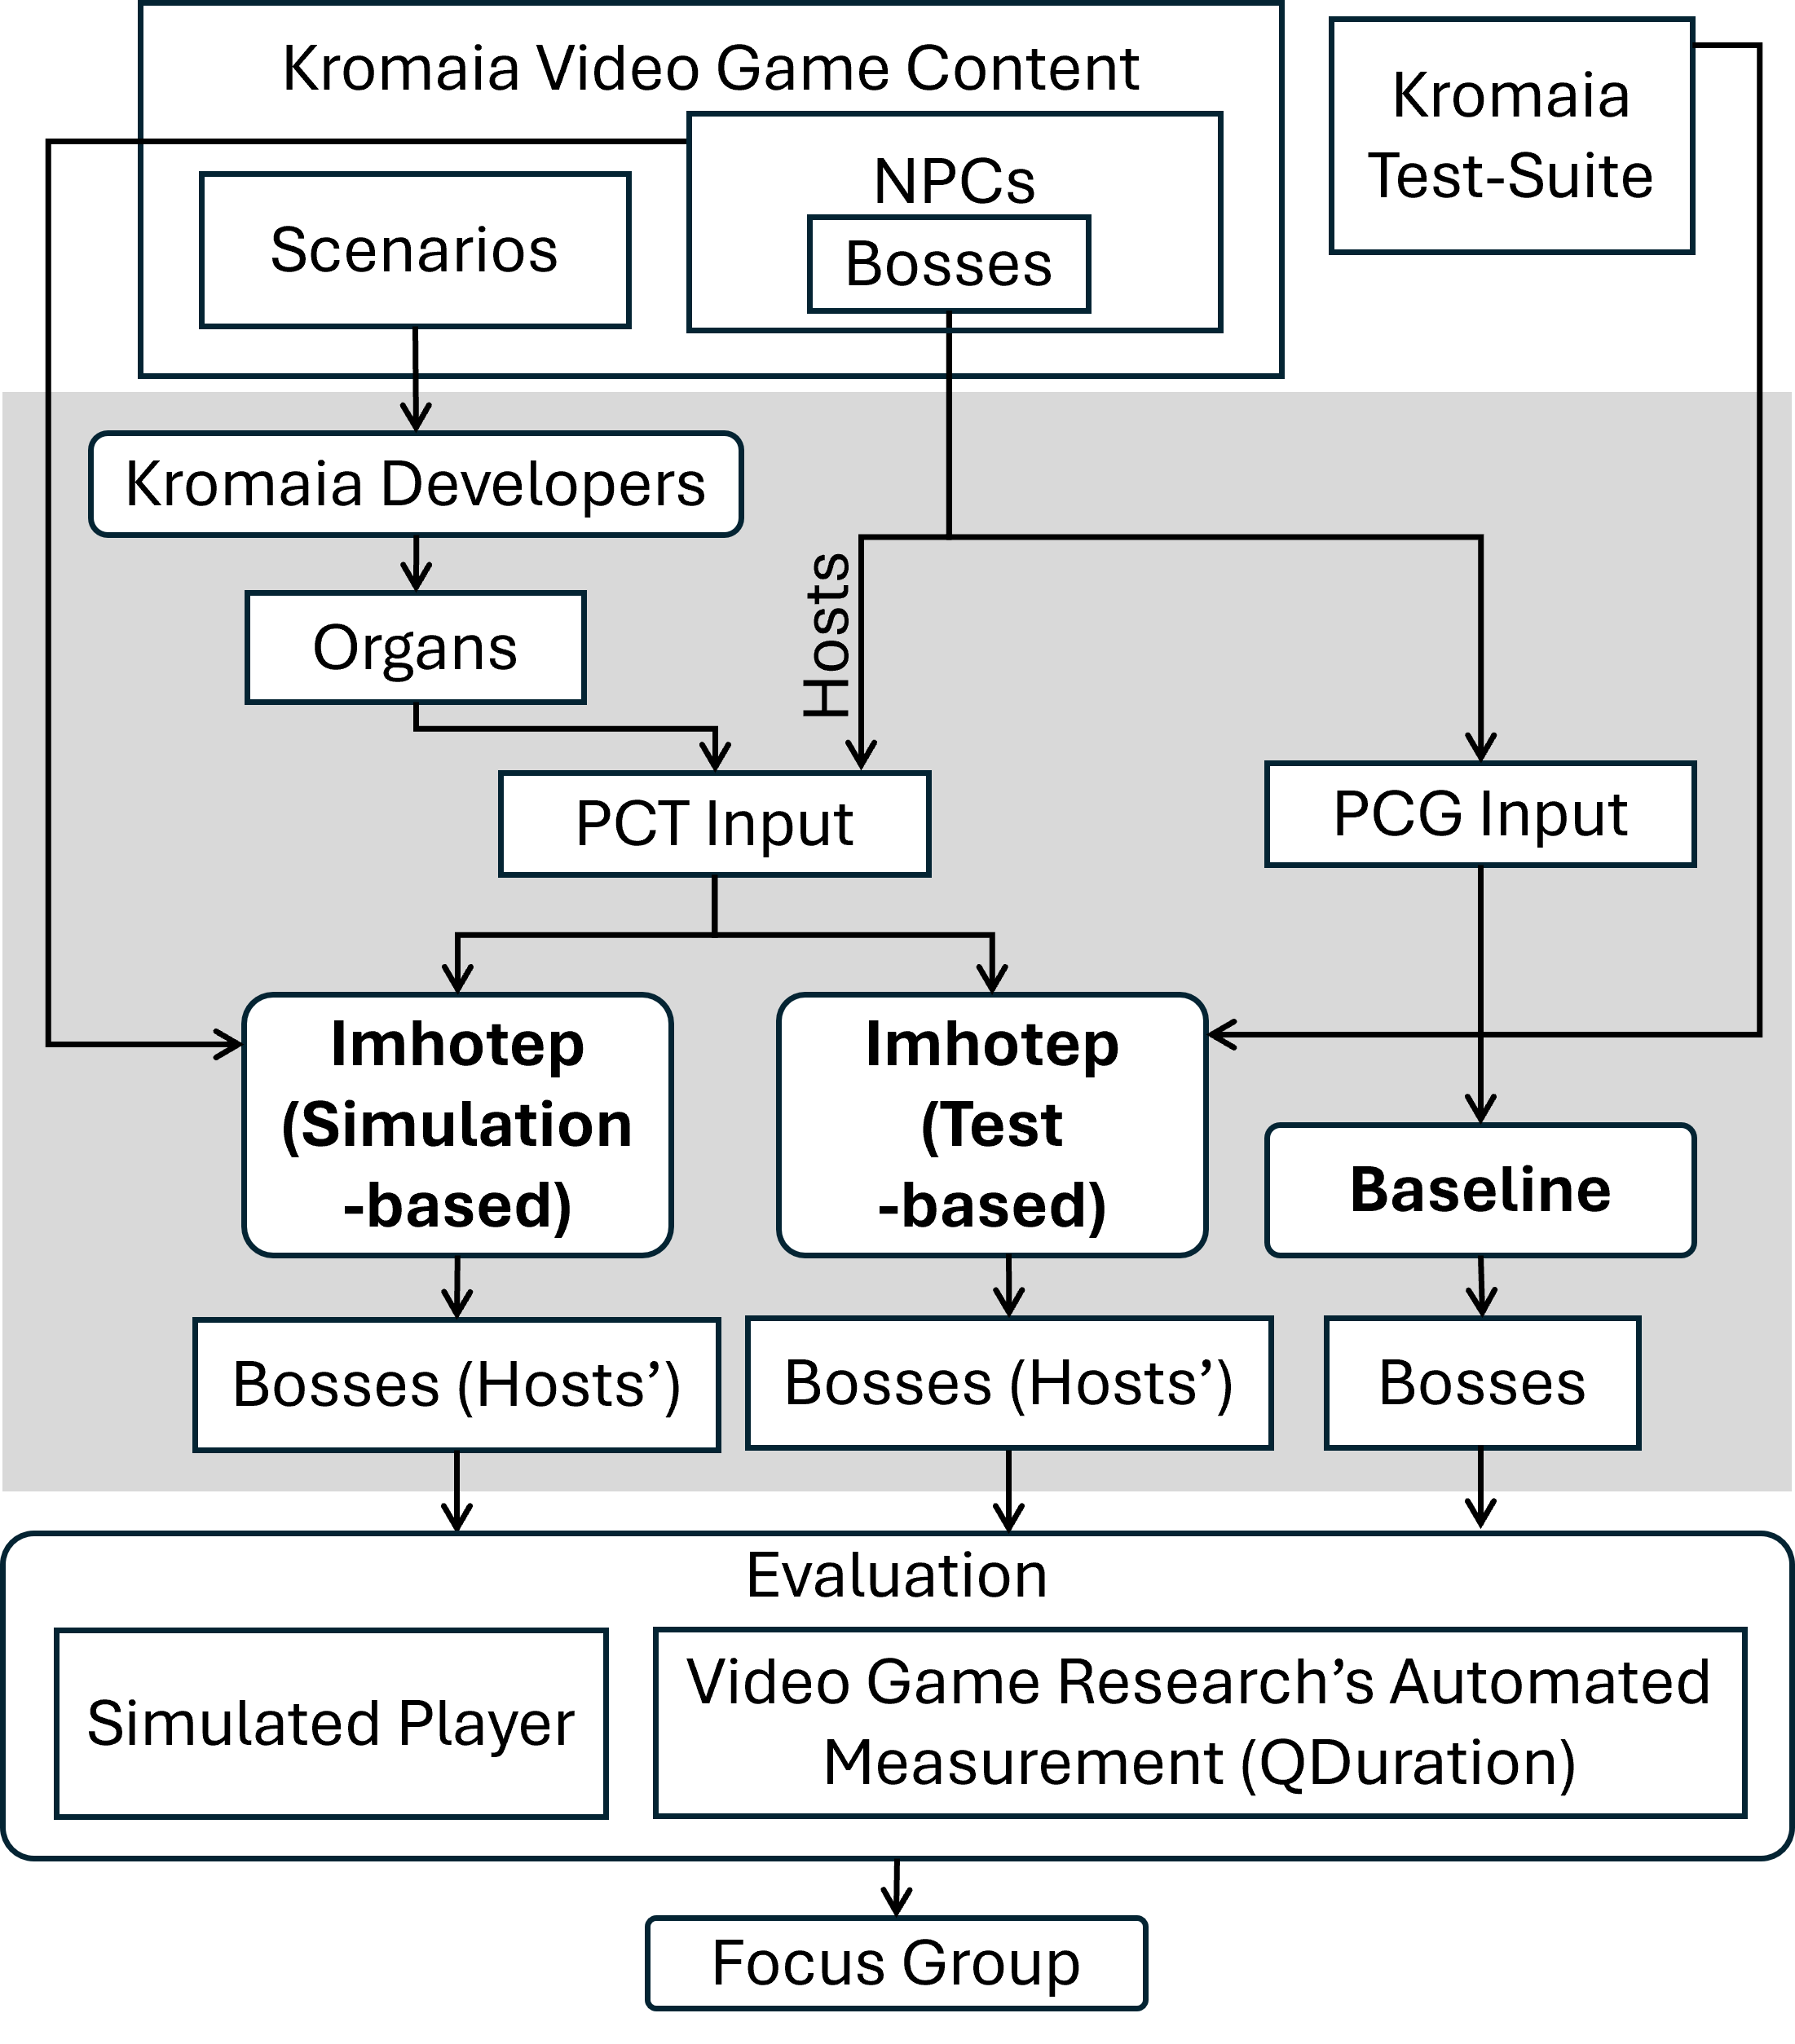
\includegraphics[width=0.4\textwidth]{Figures/evaluation_process.png}
    \caption{Overview of the evaluation process.}
    \label{fig:evaluation}
\end{figure}

\subsection{Implementation details}

We chose the parameters shown in Table~\ref{tab:evaluation_parameters} to calibrate our \ApproachName{} approach. We established the stop condition at 2 minutes and 30 seconds, ensuring that the approaches run long enough to obtain suitable solutions. The focus of this paper is not to tune the values to improve the performance of the approaches when applied to a specific problem, but rather to compare the performance of the approaches in terms of solution quality on a level playing field.

The evaluation of \ApproachName{} and the baseline was done using two PCs with the following specifications; Intel Core i7-8750H, 16GB; and  2x Intel(R) Xeon(R) CPU X5660, 64GB.
The implementation uses the Java(TM) SE Runtime Environment (JDK 1.8), together with Java as the programming language. 
For purposes of replicability and extension of our work, the implementation source code and the data are publicly available at the following URL: \url{https://anonymous.4open.science/r/Imhotep/}

\begin{table}[h]
    \centering    
    \caption{\ApproachName{} parameter settings}
    \begin{tabular}{ll}
        \hline
        \bf{Parameter description}            & \bf{Value}  \\ \hline
        Stop Criterion                   & 2m 30s \\
        Population size                  & 100    \\
        Number of parents                & 2      \\
        Number of offspring              & 2      \\
        Crossover probability            & 1      \\
        Mutation probability             & 1/150 \\ \hline
    \end{tabular}

    \label{tab:evaluation_parameters}
    \end{table}

% \subsection{Quality measurements}
% \label{subsec:Measurements}

% In a recent research done by Browne et al., the experimentation with game users showed that the following criteria stand out as being the most important: Completion, Duration, Uncertainty, Killer Moves, Permanence, and Lead Change \cite{browne2010evolutionary}. Our evaluation measures these criteria with values in the interval [0,1].

% {\bf Completion (Viability):} A game against a boss unit should end with more conclusions (victories for either the player or the boss) than draws/ties. The criterion $Q_{Completion}$ calculates a ratio of conclusions over total duel count:
% \begin{equation}
% Q_{Completion} = \frac{Conclusions}{Duels}
% \end{equation}

%  {\bf Uncertainty (Quality):} In order to keep players engaged with a duel, neither the player nor the boss unit should get extremely close to victory or defeat too early before the duel is settled, with ($T_{d}$) being its duration. Therefore, a duel is considered to be more uncertain the longer the time until the player's or the boss unit's health levels reach a dangerous/critical status ($P_{d}$ and $B_{d}$, respectively). For each duel, $Q_{Uncertainty}$ measures the average deviation between the time at which it is detected that one of the contenders is on the verge of defeat and the time corresponding to the duration of the duel.
% \begin{equation}
% Q_{Uncertainty} =  1 - \frac{\sum\limits_{d=1}^{Duels}\frac{T_{d} - min\left ( P_{d}, B_{d} \right )}{T_{d}}}{Duels} 
% \end{equation}

% {\bf Killer Moves:}   $Q_{KMoves}$ measures the proportion of killer moves by any contender ($K$), taking into account the moves that are considered to be remarkable highlights ($H$) but that are less important than killer moves. In the video game case study, the developers considered that a highlight move happens when either the boss unit or the player experiences a decrease in health; killer moves are those that make the difference in health between the contenders reach 30\%.
% \begin{equation}
% Q_{KMoves} =  1 - \frac{\sum\limits_{d=1}^{Duels}\frac{K_{d}}{H_{d}}}{Duels} 
% \end{equation}

% {\bf Permanence:} Duels with a high permanence value are games in which the advantages given by significant actions or moves by one of the contenders are unlikely to be immediately reverted by the opponent in terms of dominance. In the video game case study, the developers considered every highlight move and killer move to be meaningful actions, with recovery moves ($R$) being those that quickly cancelled the advantages given by other previous killer or highlight moves. The criterion $Q_{Permanence}$ is measured as follows:
% \begin{equation}
% Q_{Permanence} =  1 - \frac{\sum\limits_{d=1}^{Duels}\frac{R_{d}}{H_{d}+K_{d}}}{Duels} 
% \end{equation}

% {\bf Lead Change:} The lack of lead changes indicates low dramatic value. In the video game case study, the lead is determined at any given moment by considering the contender with the highest health level. This criterion is measured taking into account those highlight or killer moves that cause the lead to change ($L$) during the course of a duel:
% \begin{equation}
% Q_{LChange} = \frac{\sum\limits_{d=1}^{Duels}\frac{L_{d}}{H_{d}+K_{d}}}{Duels} 
% \end{equation}

% $Q_{Overall}$ calculates an average quality value for a model, including all of the quality criterion studied:
% \begin{equation}
% Q_{Overall} = \frac{\sum\limits_{i=1}^{N}Q_{i}}{N}
% \end{equation}
\section{Results}
\label{sec:Results}

In this section, we present the results obtained by running \ApproachName{} and the SBPCG baseline on \CaseStudy{}.
Table~\ref{tab:resultsMeanStDevRQ12} shows the mean values and standard deviations for $Q_{Duration}$ for each \ApproachName{} variant and the SBPCG baseline, while Figure~\ref{fig:results} shows the results in form of boxplots, grouped per host (i.e., the boss of \CaseStudy{}) used in our experiment, (namely Argos, Maia, Orion, Teuthus, and Vermis) and overall (last subfigure with shaded background).  
%The last group of three boxplots, with shaded background, shows the average of all the hosts for each objective function and the baseline. 
Each boxplot is generated from the results of each host obtained from transplantation \ApproachName{} (\simhotep{} and \timhotep{}) or search-based PCG (Base). Each boxplot represents 645 values of a specific host-organ transplantation (\ApproachName{}) or 645 generations from a specific host (Baseline). Each value in the boxplot is the mean value (between the 30 independent runs) of the quality indicator ($Q_{Duration}$) for one of the transplants (\ApproachName{}) or generations (Baseline). 

We can observe that both variants (\simhotep{} and \timhotep{}) obtained better results than the SBPCG baseline (Base). Specifically, \simhotep{} yielded the best results, followed by \timhotep{} and then Base. The variants obtained an average value of 44.85\% in $Q_{Duration}$, with \simhotep{} being the variant that obtained the best results overall (53.31\% in $Q_{Duration}$). \timhotep obtained 36.39\% in the overall $Q_{Duration}$, which also outperformed the baseline. The baseline obtained the worst $Q_{Duration}$. Overall, the results reveal that leveraging simulations as objective function pays off in the context of PCT, yielding 1.5x better results than the \timhotep{} and 2.5x better results than baseline.

% \begin{table*}[tb]
% \centering
% \caption{RQ1-RQ2. Mean values and standard deviations for $Q_{Duration}$ for each approach per Host and Overall.}
% \label{tab:resultsMeanStDevRQ12}
% \resizebox{.65\textwidth}{!}{
% \begin{tabular}{@{}lrrrrrr@{}}
% \toprule
% & Argos            & Maia              & Orion            & Teuthus           & Vermis            & Overall           \\ \midrule
% \rowcolor[HTML]{C0C0C0}
% \multicolumn{1}{r}{\cellcolor[HTML]{FFFFFF}{$S_{Imhotep}$}} 
% & 43.92 $\pm$ 9.30 & 43.08 $\pm$ 12.09 & 48.86 $\pm$ 8.69 & 60.78 $\pm$ 7.38  & 69.90 $\pm$ 10.52 & 53.31 $\pm$ 14.26 \\ \midrule
% \multicolumn{1}{r}{$T_{Imhotep}$} & 32.17 $\pm$ 6.94 & 29.52 $\pm$ 9.34  & 31.41 $\pm$ 6.83 & 46.33 $\pm$ 10.54 & 42.50 $\pm$ 12.96 & 36.39 $\pm$ 11.72 \\ \midrule
% \multicolumn{1}{r}{Baseline} & 20.15 $\pm$ 1.86 & 8.43 $\pm$ 1.81   & 32.97 $\pm$ 0.85 & 19.53 $\pm$ 1.88  & 25.48 $\pm$ 3.31  & 21.31 $\pm$ 8.32  \\ \bottomrule
% \end{tabular}
% }
% \end{table*}

When analysing whether there is statistical significant differences among the results obtained by \simhotep{} and Base. We found that the obtained $p-values$ for $Q_{Duration}$ are always lower than $4.01x10^{-23}$  (see Table \ref{tab:resultsWilcEffRQ1}). This is below the significance threshold value, so we can comfortably state that \simhotep{} provides significant better values for $Q_{Duration}$ with respect to Base. We also observe that all the  A12 effect size values are large (see Table \ref{tab:resultsWilcEffRQ1}), thus confirming the practical magnitude of such a difference. Thus, we conclude that:

\noindent \textbf{Answer to RQ$_1$} \simhotep{} performance far surpasses the baseline with statistically significant results and large effect size in all cases, and exhibiting a remarkable overall enhancement of 250\%.

\begin{table}[tb]	
\caption{RQ1. Mann-Withney U pair-wise test results / Vargha-Delaney Â$_{12}$ effect sizes obtained comparing \simhotep{} Vs. Base per host and overall. Â$_{12}$: Large -- L.}
	\label{tab:resultsWilcEffRQ1}
\begin{subtable}{.48\columnwidth}
    \centering
    \resizebox{\columnwidth}{!}{
	\begin{tabular}{@{}lcc@{}}
		\toprule
        & RQ1 & RQ2  \\ \cmidrule(l){2-3} 
		Boss    & $p-Value$ / Â$_{12}$    & $p-Value$ / Â$_{12}$\\ \midrule 
		Argos   & $3.25x10^{-23}$  / 0.99 (L)  & $1.28x10^{-18}$ / 0.85 (L) \\
		Maia    & $3.25x10^{-23}$  /  1.0 (L)  & $6.64x10^{-18}$ / 0.85 (L)  \\
		Orion   & $4.01x10^{-23}$  / 0.98 (L)  & $4.95x10^{-22}$ / 0.95 (L)\\
		Teuthus & $3.25x10^{-23}$  /  1.0 (L)  & $3.60x10^{-18}$ / 0.87 (L)  \\
		Vermis  & $3.25x10^{-23}$  /  1.0 (L)  & $8.86x10^{-23}$ / 0.95 (L)  \\
		Overall & $1.41x10^{-107}$ / 0.98 (L)  & $6.58x10^{-93}$ / 0.82 (L) \\
		\bottomrule
	\end{tabular}}
\end{subtable}
\begin{subtable}{.5\columnwidth}
    \centering
    \resizebox{\columnwidth}{!}{
	\begin{tabular}{@{}lccc@{}}
		\toprule  & \simhotep{} & \timhotep{} & Base        \\ \cmidrule(l){2-4} 
		Boss & Mean $\pm$ StDev & Mean $\pm$ StDe & Mean $\pm$ StDe  \\ \midrule 
		Argos  & 43.92 $\pm$ 9.30  & 32.17 $\pm$ 6.94 & 20.15 $\pm$ 1.86 \\
		Maia  & 43.08 $\pm$ 12.09  & 29.52 $\pm$ 9.34 & 8.43 $\pm$ 1.81   \\
		Orion  & 48.86 $\pm$ 8.69 & 31.41 $\pm$ 6.83 & 32.97 $\pm$ 0.85 \\
		Teuthus & 60.78 $\pm$ 7.38  & 46.33 $\pm$ 10.54 & 19.53 $\pm$ 1.88  \\
		Vermis   & 69.90 $\pm$ 10.52 & 42.50 $\pm$ 12.96 & 25.48 $\pm$ 3.31  \\
		Overall & 53.31 $\pm$ 14.26 & 36.39 $\pm$ 11.72 & 21.31 $\pm$ 8.32   \\
		\bottomrule
	\end{tabular}}
\end{subtable}
\end{table}

% \begin{table}[tb]
% 	\centering
% 	\caption{RQ1. Mann-Withney U pair-wise test results / Vargha-Delaney Â$_{12}$ effect sizes obtained comparing \simhotep{} Vs. Base per host and overall. Â$_{12}$: Large -- L.}
% 	\label{tab:resultsWilcEffRQ1}
% 	\resizebox{\columnwidth}{!}{
% 	\begin{tabular}{@{}lccccc@{}}
% 		\toprule
%         & RQ1 & RQ2   & \simhotep{} & \timhotep{} & Base        \\ \cmidrule(l){2-6} 
% 		Boss    & $p-Value$ / Â$_{12}$    & $p-Value$ / Â$_{12}$  & Mean $\pm$ StDev & Mean $\pm$ StDe & Mean $\pm$ StDe  \\ \midrule 
% 		Argos   & $3.25x10^{-23}$  / 0.99 (L)  & $1.28x10^{-18}$ / 0.85 (L) & 43.92 $\pm$ 9.30  & 32.17 $\pm$ 6.94 & 20.15 $\pm$ 1.86 \\
% 		Maia    & $3.25x10^{-23}$  /  1.0 (L)  & $6.64x10^{-18}$ / 0.85 (L) & 43.08 $\pm$ 12.09  & 29.52 $\pm$ 9.34 & 8.43 $\pm$ 1.81   \\
% 		Orion   & $4.01x10^{-23}$  / 0.98 (L)  & $4.95x10^{-22}$ / 0.95 (L)  & 48.86 $\pm$ 8.69 & 31.41 $\pm$ 6.83 & 32.97 $\pm$ 0.85 \\
% 		Teuthus & $3.25x10^{-23}$  /  1.0 (L)  & $3.60x10^{-18}$ / 0.87 (L) & 60.78 $\pm$ 7.38  & 46.33 $\pm$ 10.54 & 19.53 $\pm$ 1.88  \\
% 		Vermis  & $3.25x10^{-23}$  /  1.0 (L)  & $8.86x10^{-23}$ / 0.95 (L)  & 69.90 $\pm$ 10.52 & 42.50 $\pm$ 12.96 & 25.48 $\pm$ 3.31  \\
% 		Overall & $1.41x10^{-107}$ / 0.98 (L)  & $6.58x10^{-93}$ / 0.82 (L)  & 53.31 $\pm$ 14.26 & 36.39 $\pm$ 11.72 & 21.31 $\pm$ 8.32   \\
% 		\bottomrule
% 	\end{tabular}
% }
% \end{table}

% \begin{table}[tb]
% 	\centering
% 	\caption{RQ1. Mann-Withney U pair-wise test results / Vargha-Delaney Â$_{12}$ effect sizes obtained comparing \simhotep{} Vs. Base per host and overall. Â$_{12}$: Large -- L.}
% 	\label{tab:resultsWilcEffRQ1}
% 	\resizebox{.5\columnwidth}{!}{
% 	\begin{tabular}{@{}lrr@{}}
% 		\toprule
%         & RQ1 & RQ2          \\ \cmidrule(l){2-3} 
% 		Boss    & $p-Value$ / Â$_{12}$    & $p-Value$ / Â$_{12}$        \\ \midrule 
% 		Argos   & $3.25x10^{-23}$  / 0.99 (L)  & $1.28x10^{-18}$ / 0.85 (L)   \\
% 		Maia    & $3.25x10^{-23}$  /  1.0 (L)  & $6.64x10^{-18}$ / 0.85 (L)   \\
% 		Orion   & $4.01x10^{-23}$  / 0.98 (L)  & $4.95x10^{-22}$ / 0.95 (L)   \\
% 		Teuthus & $3.25x10^{-23}$  /  1.0 (L)  & $3.60x10^{-18}$ / 0.87 (L)   \\
% 		Vermis  & $3.25x10^{-23}$  /  1.0 (L)  & $8.86x10^{-23}$ / 0.95 (L)    \\
% 		Overall & $1.41x10^{-107}$ / 0.98 (L)  & $6.58x10^{-93}$ / 0.82 (L)    \\
% 		\bottomrule
% 	\end{tabular}
% }
% \end{table}

% \begin{table}[tb]
%     \centering
%     \caption{RQ2. Mann-Withney U pair-wise test results / Vargha-Delaney Â$_{12}$ effect sizes obtained comparing \simhotep{} Vs. \timhotep{} per host and overall. Â$_{12}$: Large -- L.}
% 	\label{tab:resultsWilcEffRQ2}
% 	\resizebox{.4\columnwidth}{!}{
%     \begin{tabular}{@{}lr@{}}
%     \toprule
%     Boss    & $p-Value$ / Â$_{12}$           \\ \midrule 
%     Argos   & $1.28x10^{-18}$ / 0.85 (L)     \\
%     Maia    & $6.64x10^{-18}$ / 0.85 (L)     \\
%     Orion   & $4.95x10^{-22}$ / 0.95 (L)     \\
%     Teuthus & $3.60x10^{-18}$ / 0.87 (L)     \\
%     Vermis  & $8.86x10^{-23}$ / 0.95 (L)     \\
%     Overall & $6.58x10^{-93}$ / 0.82 (L)     \\
%     \bottomrule
%     \end{tabular}
% }
%     \end{table}
    
As for the comparison between \simhotep{} and \timhotep{} (RQ2),  we observe that all the $p-values$ achieved when comparing the $Q_{Duration}$ distributions provided by the two \ApproachName{} variants are smaller than the significance threshold, thus indicating that the difference in solution quality is statistically significant in favour of \simhotep{}, and always with a large A12 effect size (see Table \ref{tab:resultsWilcEffRQ2}). Therefore, we conclude that:

\noindent  \textbf{Answer to RQ$_2$} \simhotep{} provides significantly better results than \timhotep{} in the context of automated content generation through transplantation, with a large effect size in all cases examined. The efficacy of \simhotep{} demonstrates a 150\% enhancement overall compared to the outcomes of \timhotep{}.

\begin{figure*}[tb]
    \centering
    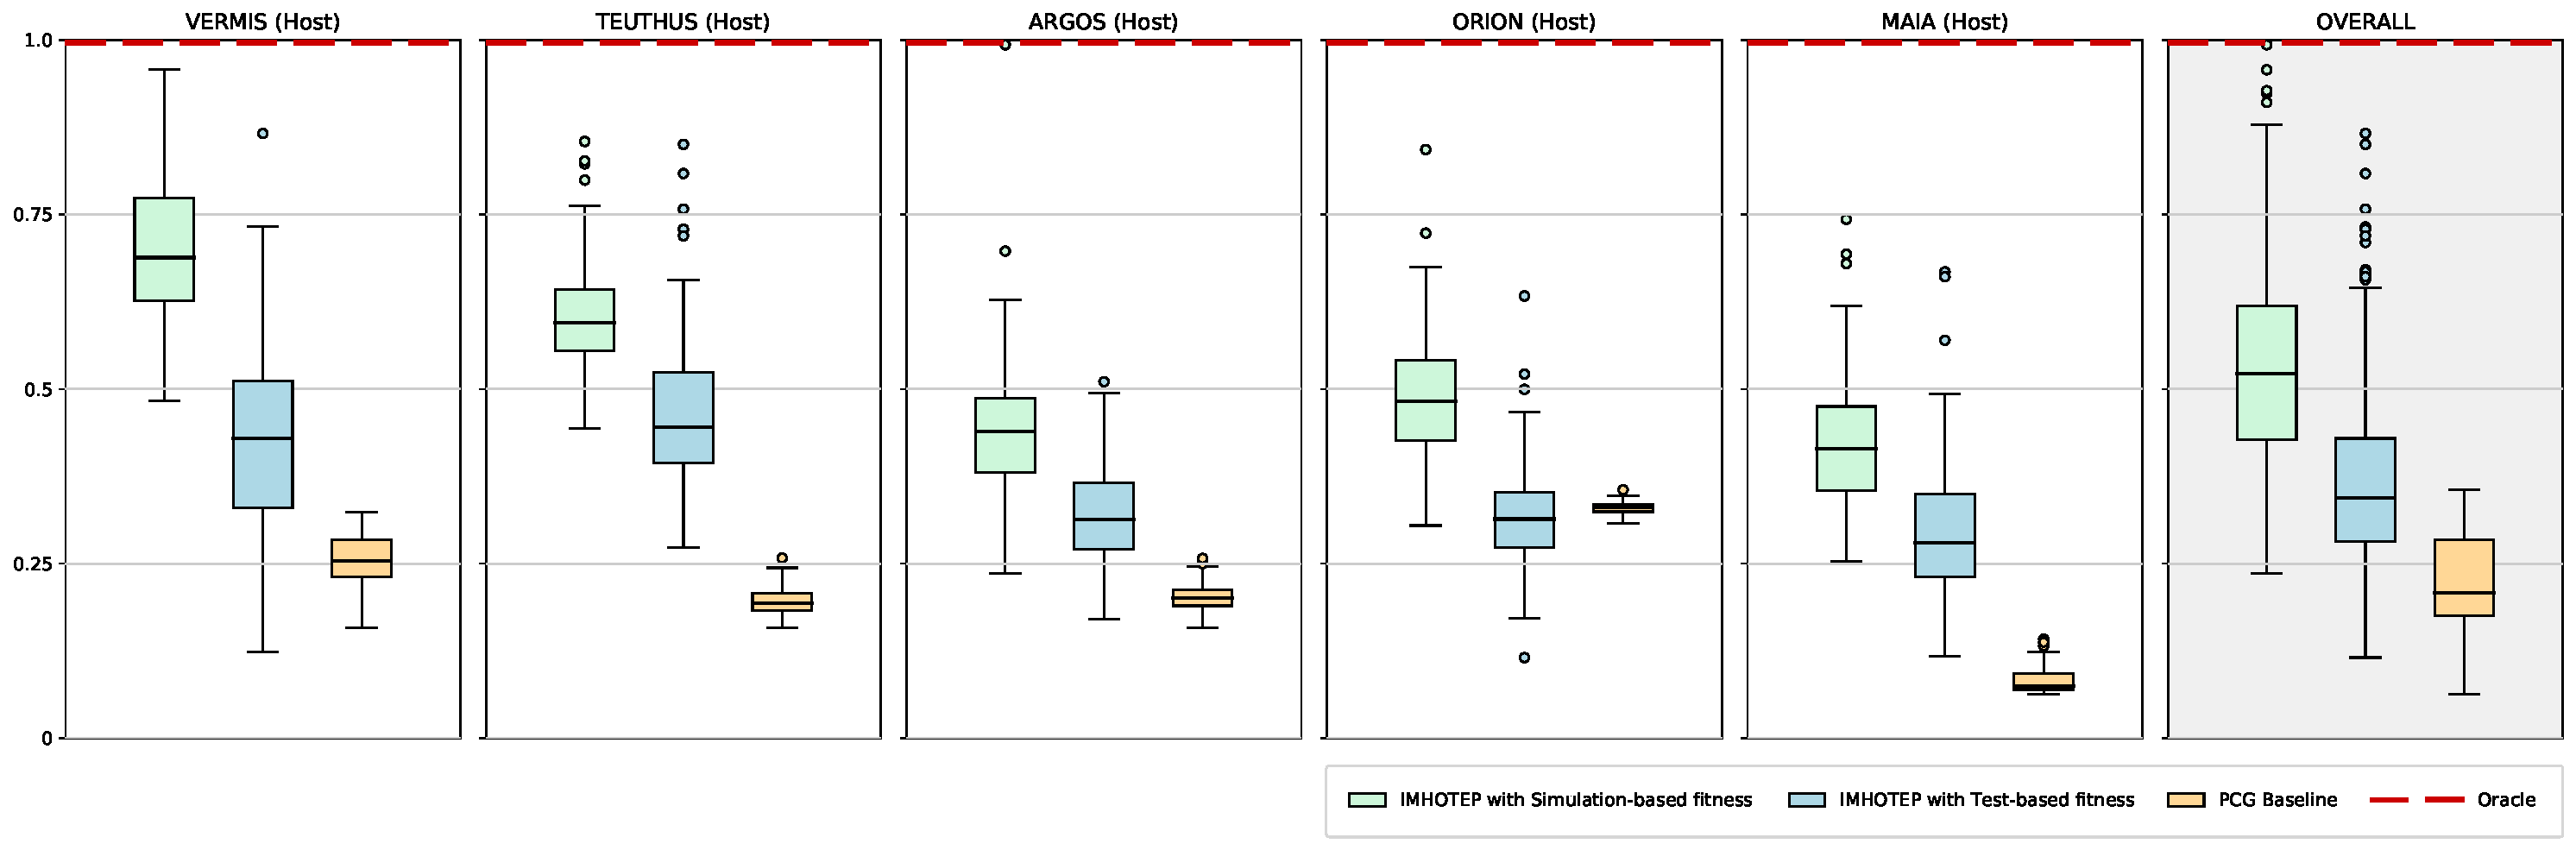
\includegraphics[width=0.8\textwidth]{Figures/Imhotep_with_legend_and_oracle_average-v4.pdf}
    \caption{RQ1-RQ2. Results of our \ApproachName{} (simulation-based and test-based) and the SBPCT baseline for the quality measurement ($Q_{Duration}$) for each of the \CaseStudy{} Host and Overall.}
    \label{fig:results}
\end{figure*}
\section{Discussion}
\label{sec:Discussion}

% The results presented in the previous section highlight that both variants of \ApproachName{} outperform the baseline. In particular, the variant of \ApproachName{} that works with a simulation-based fitness achieves better results than the rest of the evaluated approaches. The generated bosses are a suitable starting point: developers can either include them directly in the game, modify them to better suit their needs, or inspect them to look for novelties from which they can create more original designs. However, after a thorough inspection of the results, we believe that there is room for improvement within this promising line of work. To that extent, we identified a series of issues that are impacting the results, and also conducted a focus group to gather the stance of the developers with regard to the outcomes of our research.

To begin with, our work revolves around the transplantation of organs between two very different types of content in video games: scenarios and bosses. One may wonder why not transplanting organs between contents of the same type, such as between bosses. Technically, it should also be a smaller challenge to transplant organs among the same type of content due to the similarities and shared structures. However, video games put the focus on fun, which is many times achieved by avoiding repetition. Since the number of bosses is usually very limited in video games, transplanting between bosses could lead to repetition, hurting fun and creating negative play experiences for the players. In contrast, scenarios provide an abundant and promising source of organs that can withstand repetition, since it is frequent for a relevant portion of a scenario to not be explored by a player during a game: while players spend most of the time playing within scenarios, the focus of scenarios on completing goals combined with their sheer extension renders them difficult to explore in full. Hence, reusing between bosses and scenarios is more original and relevant for fun. As future work, we will also explore conducting transplants between contents of different games.

Since transplanting an organ to a host contributes to generating new desirable content, one might consider performing more than one transplant on the same host to continue creating novel content. In its current state, our approach allows for only one organ to be transplanted at a time, but it should be possible to repeatedly transplant the same organ onto the same host, or to consider chains of transplants where desirable combinations of organs can be identified and transplanted in bulk into a host. However, upon analyzing the results, we have detected various interactions between organs that may help guide an approach that considered multiple transplants: 

\begin{itemize}
    
    \item \textbf{Organ dependencies} occur when an organ requires for another organ to be present in the host to work properly. For instance, a spike weapon must be mounted on a hull belonging to the body of a boss and cannot appear by itself. In other words, a spike weapon organ depends on the existence of a hull organ to be able to be included in the boss.
    
    \item \textbf{Organ incompatibilities} happen when an organ should not appear in the host under any circumstances. For instance, consider attaching a black hole organ to a hull belonging to the boss. The black hole organ destroys everything it touches, so it would instantly end the boss without triggering the end condition for the game, since the battle is considered as completed only when the player is the one responsible for ending the boss. This would actively block player progress, which is undesirable for the game.
    
    \item \textbf{Organ synergies} are found when the functionality of an organ benefits from the existence of another organ in the host. For instance, adding one or more weapons to a hull where a weak spot is located protects the boss from the player, building a more interesting challenge.
    
    \item \textbf{Organ discordances} take place when the functionality of an organ is hindered by the existence of another organ in the host. For instance, annexing a hull with a mobile arm to another hull with a laser may cause the laser beam to be intermittently blocked, decreasing its attack capabilities.
    
\end{itemize}

So far, the literature on software transplantation does not tackle or even identify interactions between organs. Studying these organ interactions is a promising line of work to advance the concept of  transplantation both in video games and in the general software domain.

Concerning the focus group (see the bottom part of Figure.~\ref{fig:evaluation}), we conducted a survey with two developers from Entalto\footnote{https://www.entaltostudios.com/} and two from Kraken Empire\footnote{https://www.krakenempire.com/}. All of them are seasoned video game developers who devote most of their working hours to the software behind the games. We openly asked about their content preferences, presenting them with generated content whose origin (that is to say, generated by either \ApproachName{} or by the baseline) was masked, and there was unanimous preference for \ApproachName{}-generated content. 

Furthermore, they indicated that they would use it as primary content for the game rather than secondary. Primary content is that which conforms an essential part of the experience of the players, while secondary content is that which does not directly affect the main experience but contributes to creating the atmosphere of the game (for instance, distant decoration). Until now, PCG works generated results used as secondary content. In that sense, the possibility of using generated content as primary content represents an advancement in PCG. Developers justify this choice by arguing that the content generated by \ApproachName{} aligns better with the vision of the game, whereas the baseline-generated content feels more random in purpose even when reusing content that was created within the context and vision of the game by the developers.

% Finally, it is important to highlight that the simulation is not developed ad-hoc for \ApproachName{}, but rather reuses NPCs developed for the game in the simulation. In the Kromaia case study, a game within the shooting genre, NPCs are the bosses the player faces upon the end of the scenarios. This strategy of NPC reuse could be applied to other video game genres which also use NPCs that could be used for simulation purposes, such as FPS games with bots, racing games with rival competitors, or strategy games with enemy generals commanding troops faced by the player.
\section{Threats to Validity}
\label{sec:Threats}

To tackle possible threats to the validity of our work, we follow the classification suggested by De Oliveira \etal~\cite{oliveira2011threats}.

 \textbf{Conclusion Validity.}
To minimize \textit{not accounting for random variation}, we run each of the approach (\ie \simhotep, \timhotep and SBPCG) 30 times. Also, we make sure to assess the same number of solutions (\ie 645 new bosses) for each of the approaches, so to make the comparison fair. In order to address the \textit{lack of good descriptive statistics}, we present the standard deviation and a box-plot of the results. We also applied statistical significance tests (Mann-Whitney U) and effect size measurements ($\hat{A}_{12}$) following accepted guidelines~\cite{arcuri2013parameter}. We tackled the \textit{lack of a meaningful comparison baseline} by comparing \ApproachName{} to a recent and most relevant Search-Based PCG approach as a benchmark, as detailed in Section \ref{fig:evaluation}. 

\noindent \textbf{Internal Validity.}
%To mitigate \textit{poor parameter settings} we have presented the parameters used in our experiment, and for the PCG baseline we have used the parameters presented by the original work.
We provide the source code and the artefacts used in our experiments to allow for reproduction and replication, as suggested to avoid the \textit{lack of discussion on code instrumentation}.
We handled the \textit{lack of real problem instances} by using a commercial video game as the case study for our evaluation and by working closely with its developers in a real-world industrial setting. 
Likewise, the problem artefacts (donor, organs and hosts) were directly obtained from the video game developers and the documentation itself. 

\noindent \textbf{Construct Validity.}
To prevent the \textit{lack of assessing the validity of cost measures}, we made a fair comparison between the two variants of our approach and the SBPCG benchmark. Furthermore, we used a metric for the evaluation that has been widely adopted and \textit{validated} by the research community~\cite{browne2010evolutionary}.
%To mitigate the \textit{lack of discussing the underlying model subjected to optimization}, we use the original SDML of the video game provided by the developers of \CaseStudy{}.

\noindent \textbf{External Validity.}
To mitigate the lack of \textit{generalization} threat, we designed our approach to be generic and applicable not only to our industrial case study but also for generating content in other different video games. 
To avoid the \textit{lack of a clear object selection strategy} in our experiment, we have selected the instances from a commercial video game, which represents real-world instances.
In fact, \ApproachName{} can be applied where NPCs are available. NPCs are usually available in popular game genres such as car games (rival drivers), FPS games (bots), or RTS games (rival generals). For those cases were there is no NPC, the developers should ponder the trade-off of the cost of developing the NPCs and the benefits of generating content with our approach. Our approach should be replicated with other video games before assuring its generalization.


%o [+] Lack of evaluations for instances of growing size and complexity:Software Engineering techniques are designed to handle systems and teams that may vary in size and complexity. For instance, while a given software project may have a few requirements, other may have thousands. Therefore, a SBSE approach must be evaluated across a breadth of problem instances, both varying in size and complexity, to provide an assessment on the limits of the new technique.
\section{Related work} 
\label{sec:Related}

This work generates content in video games leveraging software transplantation. In this section, we discuss: (1) work that tackles automated software transplantation; and (2) work that tackles video game content generation.

\subsection{Automated Software Transplantation}

On functionality transplantation, Miles \etal~\cite{miles2012situ} and Petke \etal~\cite{petke2014using} proposed the first approaches that transplant software code in a same program (assuming that different versions of the programs are considered a same program). When transplanting within the same program, there is no need for adapters: alterations in organ or host to adapt the organ in the host. Sidiroglou-Douskos \etal~\cite{sidiroglou2015horizontal} proposed a technique that divides the donor program by specific functionality, each piece is called a \sq{shard}. The approach insert the shard into the host without modifications, that is, the work from Sidiroglou-Douskos does not use adapters either.

On the other hand, Maras \etal~\cite{maras2015towards} proposed a three step general approach, without implementing it, which applies feature localization to identify the organ; then code analysis and adaptation, and finally feature integration. Wang \etal~\cite{wang2016hunter} instead of using feature localization, takes as inputs the desired type signature of the organ and a natural language description of its functionality. With that, the approach called Hunter uses any existing code search engine to search for a method to transplant in a database of software repositories. Further, Hunter generates adapter functions to transform the types from the desired type signature into the type signatures of the candidate functions.

Allamanis \etal's SMARTPASTE~\cite{allamanis2017smartpaste} presents a different strategy to adapt the organ into the host. SMARTPASTE takes the organ and replace variable names with holes, the approach using a deep neural network fills the holes. Allamanis \etal~\cite{allamanis2017smartpaste} use Gated Graph Neural Networks~\cite{li2015gated} to predict the correct variable name in an expression.

In 2018, Lu \etal~\cite{lu2018program} introduced program splicing, a framework to automate the process of copy, paste, and organ modification. In their approach, unlike Allamanis \etal, who puts holes into the organ, the host is provided with a draft of the code with holes, or natural language comments. Similarily to, Wang \etal, program splicing looks into a database of programs to identify a relevant code to the current transplant task. Finally, the approach selects the more suitable result found to fill the holes in the draft.

$\mu$SCALPEL~\cite{barr2015automated} is an automatic code transplant tool that uses genetic programming and testing to transplant code from one program to another. $\mu$SCALPEL uses test cases to define and maintain functionalities, small changes are made to the transplanted code, and code that does not aid in passing tests can be discarded, reducing the code to its minimal functioning form. $\tau$SCALPEL~\cite{marginean2021automated} achieves the transplantation between different programs and programming languages. 

We have seen so far that Automated Software Transplantation transplants within the same platform. However, Kwon \etal propose CPR~\cite{kwon2017cpr} that transplants an entire program between different platforms. CPR realizes software transplantation by synthesizing a platform independent program from a platform dependent program. To synthesis the platform independent program, CPR uses PIEtrace~\cite{kwon2013pietrace} to construct a set of trace programs, which captures the control flow path and the data dependencies observed during a concrete execution, and replaces all the platform dependencies with the concrete values that it observed during the concrete execution. Finally, CPR merges all these trace programs together to handle any input, by replacing the concrete values observed during the executions, with input variables. 

To the best of our knowledge our is the first proposal addressing automated software transplantation in the field of content generation for video games. Our proposal allows the transplantation between different types of content. We have demonstrated that in this context the simulations yield superior outcomes compared to the test-based objective function that previously attained the most favourable results in traditional software engineering transplantation ($\mu$SCALPEL).

\subsection{Procedural Content Generation}

Procedural Content Generation (PCG) refers to the automation or semi-automation of the generation of content in video games~\cite{hendrikx2013procedural}. The types of content generated by PCG are diverse, such as vegetation~\cite{mora2021flora}, sound~\cite{plans2012experience}, terrain~\cite{frade2009breeding}, Non-Playable Characters (NPCs)~\cite{viana2022illuminating}, dungeons~\cite{viana2019survey}, puzzles~\cite{de2019procedural}, and even the rules of a game~\cite{browne2008automatic}. PCG is a large field spanning many algorithms~\cite{yannakakis2018artificial}, which can be grouped in three main categories according to the survey of PCG techniques by Barriga et al.~\cite{Barriga2019}: Traditional methods~\cite{freiknecht2017survey} that generate content under a procedure without evaluation; Machine Learning methods (PCGML)~\cite{Summerville2018,liu2021deep,souchleris2023reinforcement} that train models to generate new content; and Search-Based methods (SBPCG)~\cite{hendrikx2013procedural,togelius2011search} that generate content through a search on a predefined space guided by a meta-heuristic using one or more objective functions. 

%An interesting aspect of SBPCG is the objective function (or fitness function) that guides the search towards an optimal solution. SBPCG differentiates between three different types~\cite{togelius2011search}: direct, simulation, and interactive. Direct objective functions are those that are based on the available knowledge of developers (that is, the developers themselves participate in the assessment of the objective function). Direct objective functions can be either theory-driven (meaning that the opinion of the developers is directly leveraged) or data-driven (meaning that information about relevant parameters is extracted from artefacts like questionnaires or player models). Simulation objective functions replicate real situations to estimate the behaviour of real players. Work in this area focuses mainly on developing more human-like agents, bots, and AIs to be used as objective functions. Simulation objective functions can be static, where the simulator agent does not change during the simulation, or dynamic, where agents that learn during simulation are used. Finally, interactive objective functions are those that involve players in the composition of the objective function.In SBPCG, interactive objective functions can be either explicit, when players are outright asked for their opinions, or implicit, when the data is indirectly extracted or inferred from the observation of the actions of the players and the results of those actions.

Our work generates content of the NPC type. In the context of NPC generation using SBPCG, Ripamonti \etal~\cite{ripamonti2021dragon} developed a novel approach to generate monsters adapted to players, considering the monster with more death rate the preferred by the player. To evaluate the monsters, they recreated an environment with the main aspects from a MMORPG~\footnote{Massive Multiplayer Online Role-Playing Games} game. Pereira \etal~\cite{pereira2021procedural_enemies} and later extended by Viana \etal~\cite{viana2022illuminating} seek for generating enemies that meet a difficulty criteria. Pereira \etal and Viana \etal use the same research academic game in their experimental designs. 
Blasco \etal~\cite{blasco2021evolutionary} focusses on generating spaceship enemies that are comparable to the ones manually created by developers. To generate spaceships, Gallota \etal~\cite{gallotta2022evolving} used a combination of Lindenmayer systems~\cite{lindenmayer1968mathematical} and evolutionary algorithm. Gallota \etal as well as Blasco \etal use a commercial video game in their evaluation.


\todo{cite any recent ML and NPCs, simplifications or academics?}

The motivation of our work comes from the limitations that we detected in previous work. Previous work focused on speeding up development time. However, the influence of the developers on the generated content was limited. The generated content depended on randomness resulting on generated content not aligned with the intention of the developers. As a result, the generated content was either not used or used as secondary content. 

Our work is the first approach that tackles automated software transplantation if the field of video games. Furthermore, our proposal allows the transplantation between different types of content. More precisely, in this work, we transplant organs from a scenarios to an NPCs.

%Our previous work also generates NPCs using SBSE~\cite{blasco2021evolutionary}. Our previous work focused on using search to speed up development time. However, in our previous work the influence of the developers on the generated content was limited. The generated NPC depended on randomness resulting on generated NPCs not aligned with the intention of the developers. As a result, the generated content was either not used or used as secondary content. In fact, the limitations of our previous work were the inspiration for moving to transplantation. The transplant-based approach of this work keeps control in the hands of the developers (who choose the organ to transplant) and helps to explore the latent content that exists in the video game.

%, our approach transplant scenario elements into a NPC to obtain a novel version of the NPC. From the best of our knowledge we are the first work applying transplantation in PCG. Guarneri \etal~\cite{guarneri2013golem} or Norton \etal~\cite{norton2017monsters}  generate NPC monsters through an evolutionary algorithm with the aim of obtaining a diversity set of new monsters. With the same goal, 

%Our research introduces a fresh perspective on content generation through the use of transplantation, which sets it apart from traditional procedural content generation (PCG) methods. Transplantation enables the seamless integration of various content types, facilitating in our work the transplant of elements from scenarios to NPCs.

% \subsection{MDE and Game Software Engineering}

% One of the challenges in software development is the environment used, as each environment and programming languages has unique characteristics. Software models, and more precisely Model Driven Engineering, study how to alleviate this problem by approaching software development from a platform-independent perspective through models. Video game developers must deal with this challenge as well and has motivated the research that combine software models and the domain of video games. 

% The 2010 survey of Software Engineering Research for Computer Games~\cite{ampatzoglou2010software} identified only one work that applied Model-Driven Development to video games~\cite{reyno2009automatic}. That work coined the term ‘‘Model-Driven Game Development’’ and presented a first approach to 2D game prototyping through Model-Driven Development. Specifically, they used UML classes and state diagrams that were extended with stereotypes, and a model-to-code transformation to generate C++ code.

% More recent work presents work that intended to minimize errors, time, and cost in multi-platform video game development and maintenance~\cite{Nunez17,Nunez13,Usman17}, or suggest the use of business process models as the modelling language for video games~\cite{Solis15}.

% In the intersection between software models and evolutionary computation, Williams \etal~\cite{Williams11} use an evolutionary algorithm to search for desirable game character behaviours in a text-based video game that plays unattended combats and that outputs an outcome result. The character behaviour is defined using a Domain-Specific Language. The combats are managed internally and are only driven by behaviour parameters, without taking into account a spatial environment, real-time representation, or visual feedback (which takes into consideration the physical interaction of the characters, variation in the properties, etc.).

% Another work that focuses on the intersection between software models and evolutionary computation is Avida-MDE~\cite{Goldsby2008}, which generates state machines that describe the behaviour of one of the classes of a software system (Adaptive Flood Warning System case study). The resulting state machines comply with developer requirements (scenarios for
% adaptation). Instead of generating whole models, Avida-MDE extends already existing models (object models and state machines) with new state machines that support new scenarios. The work in Goldsby and Cheng \etal~\cite{Goldsby2008} does not report the size of the generated state machines; however, the ones shown in the paper are around 50 model elements, which is significantly smaller than the more than 1000 model elements of the models of a commercial video game such as Kromaia.

% The work mentioned above focus on generating new content from models, which differs with our proposal of using MDE to transplant model fragments between models.

% \subsection{Conclusion}

% Our work differs from previous work for various aspects. 
% To the best of our knowledge our is the first paper addressing automated software transplantation if the field of video games. Our proposal allows the transplantation between different types of content. More precisely, we transplant elements from a scenario to an NPC. The use of MDE separate the problem from the platform, and even the specific video game, as a same Domain Specific Language can be used in different video games.
\section{Conclusion}
\label{sec:Conclusion}

%Procedural Content Generation (PCG) aims for the (semi) automatic generation of new content within video games.  Typically, current PCG methods are operated by developers providing initial content to an algorithm, which then generates additional content. However, the developers have limited control over the generation process, which results in the generated content being used as secondary content, or not been used at all.

%In this study, we empower developers by introducing the transplantation metaphor into PCG for the first time. Our approach allows game developers to choose an organ from a donor and a host that will receive the organ. Through our approach, we aim to search for a suitable solution to integrate the organ into the host. To guide our search, we propose two distinct objective functions: one based on test case following conventional software transplantation method, and another novel objective function based on simulations, proposed here.

%Our proposal has been empirically assessed by using the commercial video game \CaseStudy{}. To evaluate our approach, we have transplanted a total of 129 distinct organs from the scenarios of \CaseStudy{} into 5 video game bosses, which serve as hosts. This transplantation process has resulted in the creation of 1290 new video game bosses. We then compare the outcomes of our approach (the two variants) with a PCG baseline.

%Our \simhotep{} produces results that are 1.5 times superior to those of the \timhotep{} and 2.5 times superior to the baseline. The statistical analysis confirms the significance of these differences and highlights the substantial magnitude of improvement.
%Furthermore, a focus group with game developers indicated that first, they would use the generated content by our approach, and secondly, that they would use it as primary content for the game rather than secondary.

In this study, we empower developers by introducing the transplantation metaphor into PCG for the first time. Our approach allows game developers to choose an organ from a donor and a host that will receive the organ.
Our results demonstrate that we have successfully generated new content through transplantation. Not only that alone, we have accomplish 645 transplantation in total for a commercial video game. Furthermore, our work achieves transplantation between different types of content which results in expanding the library of organs available. This can inspire researchers and developers to explore the use of different types of content for creating new content automatically. 

In addition, we have presented a novel objective function to guide search software transplantation, which has obtained better results than traditional one. This novel search guidance opens a door in the field of software transplantation.
In fact, we identified that there is an opportunity in going beyond transplant evolution, by co-evolving transplants and simulations. We could evolve the simulations by adding or removing elements like NPCs, items, and scenarios. These co-evolutionary approaches enable developers to gain a deeper understanding of the contexts where the generated content performs better. Furthermore, this co-evolutionary approaches may empower researchers to tackle the challenge of transplanting content between different games. Achieving the former would open the door to a vast and potentially highly original catalogue of organs for transplantation that would contribute to achieving what developers seek with their video games: fun.


\bibliographystyle{IEEEtran}
\bibliography{references}

\end{document}
